% % Preamble BEGIN %%%%%%%%%%%%%%%%%%%%%%%%%%%%%%%%%%%%%%%%%%%%%%%%%%%%%%%%%

%%% Preamble (Dokumentenklasse)
% ------------------------------------------------------------------------
% LaTeX - Preambel ******************************************************
% ------------------------------------------------------------------------
% Dokumentklasse (Koma Script)
% ------------------------------------------------------------------------
% basiernd auf www.matthiaspospiech.de/latex/vorlagen Diplomarbeit kompakt
% ========================================================================
\documentclass[%
  draft=false,         % Entwurfsstadium
  % final,            % fertiges Dokument
  fontsize=12pt,      % Schriftgroesse der Grundschrift
  headings=big,       % große Überschriften
  ngerman,            % wird an andere Pakete weitergereicht
  paper=a4,           % Papierformat
  BCOR=5mm,           % Bindekorrektur: Zusätzlicher Rand auf der Innenseite
  DIV=14,             % Seitengröße (siehe Koma Skript Dokumentation !)
  1.1headlines,       % Zeilenanzahl der Kopfzeilen
  pagesize,           % Schreibt die Papiergroesse in die Datei.
  twoside=false,      % Einseitiges Layout
  % twoside,            % Zweiseitiges Layout
  openright,          % Kapitel beginnen immer auf der rechten Seite
  titlepage,          % Titel als einzelne Seite ('titlepage' Umgebung)
  headsepline,        % Linie unter Kolumnentitel ()
  % plainheadsepline,   % Linie unter Kolumnentitel () plain Seitenstil
  chapterprefix=false, % keine Ausgabe von 'Kapitel:'
  bibliography=totoc,  % Bibliographie ins TOC
  % bibtotocnumbered,   % Bibliographie ins TOC mit Kapitelnummer
  toc=graduated,      % eingereuckte Gliederung
  listof=graduated,   % eingereuckte LOT, LOF
  numbers=noenddot,   % Überschriftnummerierung ohne Punkt, siehe DUDEN !
  cleardoublepage=empty, % Leere linke Seite bei Zweiseitenlayout vor Kapitel
  fleqn,              % Formeln werden linksbuendig angezeigt
  % parindent,          % Absatz mit Einzug (Standard)
  parskip=half,       % Absatz halbe Zeile Abstand
  % parskip,            % Absatz ganze Zeile Abstand
]{scrbook}%     Klassen: scrartcl, scrreprt, scrbook


%%% Alle Namen usw. im Titel und im hyperref-Paket
% ------------------------------------------------------------------------
% LaTeX - Preambel ******************************************************
% ------------------------------------------------------------------------
% pre-work
% ========================================================================
% % ToDo kennzeichnen
\newcommand{\workTodo}[1]{\textcolor{red}{todo: #1}}

% % Für Datum und Zeit in Fusszeile
% % !!!Inhalt bei Fertigstellung der Arbeit löschen
\newcommand{\workMarkDateTime}{\today{} - \thistime\ Uhr}

% % Alle Namen werden im Titel und im hyperref-Paket eingetragen
% % !!! Ueberall für <Wert> das Entsprechende eintragen

 % <Typ> Studienarbeit, Dipolmarbeit, Studienarbeit oder Bachlor-Abschlussarbeit
\newcommand{\workTyp}{Bachlor-Abschlussarbeit\xspace}

 % <Titel> der Arbeit
\newcommand{\workTitel}{Modularising existing functionality of an enterprise monolith system into microservices\xspace}

 % <Studiengang> z.B. Kommunikationstechnik
\newcommand{\workStudiengang}{Informationstechnik}

% <Semester> mit Jahr z.B. Sommersemester 2008
\newcommand{\workSemester}{Wintersemester 2019/20}

% <Name> des Studenten
\newcommand{\workNameStudent}{Lukas Hermann}

% <Pruefer> Name des prüfenden (betreuenden) Professor an der Hochschule
\newcommand{\workPruefer}{Karin Melzer}


% %%% Nur bei Abschluss-Arbeiten

% <Datum> der Abgabe der Arbeit (Eidesstatliche Erklärung)
\newcommand{\workDatum}{\today\xspace}

% <Zweitprüfer>
\newcommand{\workZweitPruefer}{Reiner Marchthaler}

% <Zeitraum>
\newcommand{\workZeitraum}{9. Oktober 2019 – 9. Februar 2020}


% %%% Nur bei Industrie-Arbeiten:

% <Firma>
\newcommand{\workFirma}{Capgemini Service SAS}

% <Betreuer in der Firma>
\newcommand{\workBetreuer}{Robin Kurz}

% Firmenlogo Name hier anpassen, Größe (wenn möglich) nicht ändern
\newcommand{\workFirmenLogo}{
\includegraphics[width=5cm]{fig/aa-titel/capgemini_logo}}


%%% Preamble (Pakete)
% ------------------------------------------------------------------------
% LaTeX - Preambel ******************************************************
% ------------------------------------------------------------------------
% Packages
% ------------------------------------------------------------------------
% basiernd auf www.matthiaspospiech.de/latex/vorlagen Diplomarbeit kompakt
% ========================================================================

% Inhalt:
% 1. Einige Pakete muessen unbedingt vor allen anderen geladen werden
% 2. Fonts Fonts Fonts
% 3. Math Packages
% 4. Symbole
% 5. text related packages
% 6. Pakete zum Zitieren
% 7. PDF related packages
% 8. Tables (Tabular)
% 9. figures and placement
% 10. verbatim packages
% 11. science packages
% 12. layout packages

% ~~~~~~~~~~~~~~~~~~~~~~~~~~~~~~~~~~~~~~~~~~~~~~~~~~~~~~~~~~~~~~~~~~~~~~~~
% Encoding der Dateien (sonst funktionieren Umlaute nicht)
% Empfohlen latin1, da einige Pakete mit utf8 Zeichen nicht
% funktionieren, z.B: listings, soul.

% \usepackage[latin1]{inputenx} % ISO-8859-1
%\usepackage[ansinew]{inputenx} % Windows-Standard (CP1252) (baut auf ISO 8859-1 und ISO 8859-15 auf)
\usepackage[utf8]{inputenc}
% \setdefaultlanguage{english}

% ~~~~~~~~~~~~~~~~~~~~~~~~~~~~~~~~~~~~~~~~~~~~~~~~~~~~~~~~~~~~~~~~~~~~~~~~
% 1. Einige Pakete muessen unbedingt vor allen anderen geladen werden
% ~~~~~~~~~~~~~~~~~~~~~~~~~~~~~~~~~~~~~~~~~~~~~~~~~~~~~~~~~~~~~~~~~~~~~~~~
%
\usepackage{xspace} % Define commands that don't eat spaces.
\usepackage{ifpdf} % Fuer Pakete/Paketoptionen, die nur fuer pdf benoetigt werden \ifpdf \else \fi
\usepackage{calc} % Calculation with LaTeX
\usepackage[main=english,ngerman]{babel} % Languagesetting
\usepackage[table]{xcolor} % Farben
\usepackage[]{graphicx} % Bilder
\usepackage{subcaption}
%\usepackage{epstopdf} % If an eps image is detected, epstopdf is automatically called to convert it to pdf format.
\usepackage[]{amsmath} % Amsmath - Mathematik Basispaket
\usepackage{ragged2e} % Besserer Flatternsatz (Linksbuendig, statt Blocksatz)
\usepackage{scrhack}

% ~~~~~~~~~~~~~~~~~~~~~~~~~~~~~~~~~~~~~~~~~~~~~~~~~~~~~~~~~~~~~~~~~~~~~~~~
% 2. Fonts Fonts Fonts
% ~~~~~~~~~~~~~~~~~~~~~~~~~~~~~~~~~~~~~~~~~~~~~~~~~~~~~~~~~~~~~~~~~~~~~~~~

\usepackage[T1]{fontenc} % T1 Schrift Encoding (notwendig für die meisten Type 1 Schriften)
\usepackage{textcomp}  % Zusatzliche Symbole (Text Companion font extension)

% Alle Schriften die hier angegeben sind sehen im PDF richtig aus.
% Die LaTeX Standardschrift ist die Latin Modern (lmodern Paket).
% If Latin Modern is not available for your distribution you must install the
% package cm-super instead. Otherwise your fonts will look horrible in the PDF

% DO NOT LOAD ae-Package for the font !

%% - Latin Modern
\usepackage{lmodern}
%% -------------------
%
% % - Times, Helvetica, Courier (Word Standard...)
%\usepackage{mathptmx}
%\usepackage[scaled=.90]{helvet}
%\usepackage{courier}
% % -------------------
%%
%% - Palantino , Helvetica, Courier
%\usepackage{mathpazo}
%\usepackage[scaled=.95]{helvet}
%\usepackage{courier}
%% -------------------
%
%% - Bera Schriften
%\usepackage{bera}
%% -------------------
%
%% - Charter, Bera Sans
%\usepackage{charter}\linespread{1.05}
%\renewcommand{\sfdefault}{fvs}


% ~~~~~~~~~~~~~~~~~~~~~~~~~~~~~~~~~~~~~~~~~~~~~~~~~~~~~~~~~~~~~~~~~~~~~~~~
% 3. Math Packages
% ~~~~~~~~~~~~~~~~~~~~~~~~~~~~~~~~~~~~~~~~~~~~~~~~~~~~~~~~~~~~~~~~~~~~~~~~

\usepackage[fixamsmath,disallowspaces]{mathtools} % Erweitert amsmath und behebt einige Bugs
\usepackage{fixmath}
\usepackage[all,warning]{onlyamsmath} % Warnt bei Benutzung von Befehlen die mit amsmath inkompatibel sind.
\usepackage{icomma} % Erlaubt die Benutzung von Kommas im Mathematikmodus

% ~~~~~~~~~~~~~~~~~~~~~~~~~~~~~~~~~~~~~~~~~~~~~~~~~~~~~~~~~~~~~~~~~~~~~~~~
% 4. Symbole
% ~~~~~~~~~~~~~~~~~~~~~~~~~~~~~~~~~~~~~~~~~~~~~~~~~~~~~~~~~~~~~~~~~~~~~~~~
\usepackage{amssymb}
%\usepackage{wasysym}
%\usepackage{marvosym}
%\usepackage{pifont}

% ~~~~~~~~~~~~~~~~~~~~~~~~~~~~~~~~~~~~~~~~~~~~~~~~~~~~~~~~~~~~~~~~~~~~~~~~
% 5. text related packages
% ~~~~~~~~~~~~~~~~~~~~~~~~~~~~~~~~~~~~~~~~~~~~~~~~~~~~~~~~~~~~~~~~~~~~~~~~

\usepackage{url} % Setzen von URLs. In Verbindung mit hyperref sind diese auch aktive Links.
\usepackage[stable,perpage, ragged,  multiple]{footmisc} % Fussnoten
\usepackage[english]{varioref} % Intelligente Querverweise
\usepackage{enumitem} % Listen

% ~~~~~~~~~~~~~~~~~~~~~~~~~~~~~~~~~~~~~~~~~~~~~~~~~~~~~~~~~~~~~~~~~~~~~~~~
% 6. Pakete zum Zitieren
% ~~~~~~~~~~~~~~~~~~~~~~~~~~~~~~~~~~~~~~~~~~~~~~~~~~~~~~~~~~~~~~~~~~~~~~~~

\usepackage[babel, english=american, german=quotes, french=guillemets]{csquotes} % clever quotations
\SetBlockThreshold{2} % Anzahl von Zeilen
\newenvironment{myquote}%
          {\begin{quote}\small}%
          {\end{quote}}%
\SetBlockEnvironment{myquote}

\usepackage[
  backend=biber,
  style=alphabetic,
  sorting=ynt
]{biblatex}
\addbibresource{bib/main.bib}

% ~~~~~~~~~~~~~~~~~~~~~~~~~~~~~~~~~~~~~~~~~~~~~~~~~~~~~~~~~~~~~~~~~~~~~~~~
% 7. PDF related packages
% ~~~~~~~~~~~~~~~~~~~~~~~~~~~~~~~~~~~~~~~~~~~~~~~~~~~~~~~~~~~~~~~~~~~~~~~~

\ifpdf % Wenn als PDF ausgegeben wird
\usepackage{pdfpages} % pdf-Seiten einbinden
\usepackage[pdftex]{hyperref} % PDF Option in Hyperref
\else
\usepackage[dvipdfm]{hyperref}
\fi

%%% Doc: ftp://tug.ctan.org/pub/tex-archive/macros/latex/contrib/pdfpages/pdfpages.pdf
%\usepackage{pdfpages} % Include pages from external PDF documents in LaTeX documents

%%% Doc: ftp://tug.ctan.org/pub/tex-archive/macros/latex/contrib/hyperref/doc/manual.pdf
\hypersetup{
          pdfhighlight = /O,           % Visualisierung beim anklicken von Links
% Farben fuer die Links
   colorlinks=true,         % Links erhalten Farben statt Kaestchen
   urlcolor=darkblue,    % \href{...}{...} external (URL)
   filecolor=darkblue,  % \href{...} local file
   linkcolor=darkblue,  % \ref{...} and \pageref{...}
          citecolor =darkblue,    % Literaturverzeichnis
   % Links
   raiselinks=true,      % calculate real height of the link
   breaklinks,          % Links bestehen bei Zeilenumbruch
%   backref=page,          % Backlinks im Literaturverzeichnis (section, slide, page, none)
%   pagebackref=true,        % Backlinks im Literaturverzeichnis mit Seitenangabe
   verbose,
%   hyperindex=true,         % backlinkex index
   linktocpage=true,        % Inhaltsverzeichnis verlinkt Seiten
%   hyperfootnotes=false, % Keine Links auf Fussnoten
   % Bookmarks
%   bookmarks=true,          % Erzeugung von Bookmarks fuer PDF-Viewer
   bookmarksopenlevel=1,    % Gliederungstiefe der Bookmarks
   bookmarksopen=true,      % Expandierte Untermenues in Bookmarks
   bookmarksnumbered=true,  % Nummerierung der Bookmarks
   bookmarkstype=toc,       % Art der Verzeichnisses
   % Anchors
   plainpages=false,        % % Make page anchors using the formatted form of the page number. With this option, hyperref writes different anchors for pages ‘ii’ and ‘2’. (If the option is set ‘true’ — the default — hyperref writes page anchors as the arabic form of the absolute page number, rather than the formatted form.)
   % hypertexnames=false,
   pageanchor=true,         % Pages are linkable
   % PDF Informationen
   pdftitle={\workType: \workTitel},         % Titel
   pdfauthor={\workNameStudent},      % Autor
   pdfcreator={LaTeX, hyperref, KOMA-Script}, % Ersteller
   %pdfproducer={pdfeTeX 1.10b-2.1} %Produzent
   pdfstartview=FitH,       % Dokument wird Fit Width geaefnet
   pdfpagemode=UseOutlines, % Bookmarks im Viewer anzeigen
%   pdfpagelabels=true,      % set PDF page labels
}

% ~~~~~~~~~~~~~~~~~~~~~~~~~~~~~~~~~~~~~~~~~~~~~~~~~~~~~~~~~~~~~~~~~~~~~~~~
% 8. Tables (Tabular)
% ~~~~~~~~~~~~~~~~~~~~~~~~~~~~~~~~~~~~~~~~~~~~~~~~~~~~~~~~~~~~~~~~~~~~~~~~

\usepackage{booktabs}
\usepackage{tabularx} % tabularx nach hyperref laden
\usepackage{multirow}

% ~~~~~~~~~~~~~~~~~~~~~~~~~~~~~~~~~~~~~~~~~~~~~~~~~~~~~~~~~~~~~~~~~~~~~~~~
% 9. figures and placement
% ~~~~~~~~~~~~~~~~~~~~~~~~~~~~~~~~~~~~~~~~~~~~~~~~~~~~~~~~~~~~~~~~~~~~~~~~

%% Bilder und Graphiken ==================================================

\usepackage{float}  % Stellt die Option [H] fuer Floats zur Verfgung
\usepackage{flafter} % Floats immer erst nach der Referenz setzen
\usepackage{subfig} % Layout wird weiter unten festgelegt !
\usepackage{wrapfig} % Bilder von Text Umfliessen lassen

\usepackage{placeins} % Alle Floats bis \FloatBarrier ausgeben

% Make float placement easier
\renewcommand{\floatpagefraction}{.75} % vorher: .5
\renewcommand{\textfraction}{.1}       % vorher: .2
\renewcommand{\topfraction}{.8}        % vorher: .7
\renewcommand{\bottomfraction}{.5}     % vorher: .3
\setcounter{topnumber}{3}          % vorher: 2
\setcounter{bottomnumber}{2}           % vorher: 1
\setcounter{totalnumber}{5}          % vorher: 3


% ~~~~~~~~~~~~~~~~~~~~~~~~~~~~~~~~~~~~~~~~~~~~~~~~~~~~~~~~~~~~~~~~~~~~~~~~
% 10. verbatim packages
% ~~~~~~~~~~~~~~~~~~~~~~~~~~~~~~~~~~~~~~~~~~~~~~~~~~~~~~~~~~~~~~~~~~~~~~~~

%%% Doc: ftp://tug.ctan.org/pub/tex-archive/macros/latex/contrib/upquote/upquote.sty
\usepackage{upquote} % Setzt "richtige" Quotes in verbatim-Umgebung

%%% Doc: No Documentation
% \usepackage{verbatim} % Reimplemntation of the original verbatim

%%% Doc: http://www.cs.brown.edu/system/software/latex/doc/fancyvrb.pdf
% \usepackage{fancyvrb} % Superior Verbatim Class

%% Listings Paket ------------------------------------------------------
%%% Doc: ftp://tug.ctan.org/pub/tex-archive/macros/latex/contrib/listings/listings-1.3.pdf
\usepackage{listings}

\lstset{
basicstyle =\ttfamily\color{black}\small, % Standardschrift
keywordstyle =, % \bfseries\color{blue}   % Schlüsselwort-Style
%identifierstyle =\underbar,
commentstyle =\color{teal},
stringstyle =\itshape,
numbers = left,       % Ort der Zeilennummern
numberstyle =\tiny\color{black},     % Stil der Zeilennummern
numbers = left,       % Ort der Zeilennummern
tabsize=2,        % Groesse von Tabs
breaklines,       % Zeilen werden Umgebrochen
breakatwhitespace,        % An Leerzeichen umbrechen
%showspaces=true,       % Leerzeichen anzeigen
backgroundcolor=\color{lightgray},    % % Hintergrundfarbe der Listings
}
 \lstloadlanguages{% Check Dokumentation for further languages ...
% [Visual]Basic
         [AlLaTeX]TeX,
         %Pascal
         %C
         %C++
         %XML
         %HTML
 }

%%% Doc: ftp://tug.ctan.org/pub/tex-archive/macros/latex/contrib/examplep/eurotex_2005_examplep.pdf
% LaTeX Code und Ergebnis nebeneinander darstellen
%\usepackage{examplep}


% ~~~~~~~~~~~~~~~~~~~~~~~~~~~~~~~~~~~~~~~~~~~~~~~~~~~~~~~~~~~~~~~~~~~~~~~~
% 11. science packages
% ~~~~~~~~~~~~~~~~~~~~~~~~~~~~~~~~~~~~~~~~~~~~~~~~~~~~~~~~~~~~~~~~~~~~~~~~

% \usepackage[squaren]{SIunits}

% ~~~~~~~~~~~~~~~~~~~~~~~~~~~~~~~~~~~~~~~~~~~~~~~~~~~~~~~~~~~~~~~~~~~~~~~~
% 12. layout packages
% ~~~~~~~~~~~~~~~~~~~~~~~~~~~~~~~~~~~~~~~~~~~~~~~~~~~~~~~~~~~~~~~~~~~~~~~~

\usepackage{multicol}

%% Zeilenabstand =========================================================
%
%%% Doc: ftp://tug.ctan.org/pub/tex-archive/macros/latex/contrib/setspace/setspace.sty
\usepackage{setspace}
%\doublespace         % 2-facher Abstand
%\onehalfspace    % 1,5-facher Abstand
% hereafter load 'typearea' again

%% Seitenlayout ==========================================================
%
% Layout mit 'typearea'
\typearea[current]{last}
\raggedbottom     % Variable Seitenhoehen zulassen


%% Kopf und Fusszeilen====================================================
%%% Doc: ftp://tug.ctan.org/pub/tex-archive/macros/latex/contrib/koma-script/scrguide.pdf
\usepackage[%
   automark,   % automatische Aktualisierung der Kolumnentitel
   markcase=ignoreuppercase,   % Grossbuchstaben verhindern
]{scrlayer-scrpage}

\usepackage{scrtime} % Zeit
%\usepackage{scrdate} % Datum

\pagestyle{scrheadings} % Seite mit Headern
%\pagestyle{scrplain} % Seiten ohne Header
%\pagestyle{empty} % Seiten ohne Header

% loescht voreingestellte Stile
\clearscrheadings
\clearscrplain
%
% [scrplain]{scrheadings}

% %%% Kopfzeile
% einseitig: Bei einseitigem Layout, nur folgende Zeilen verwenden !!!
\ihead[]{\leftmark} % links: Kapitel
 %\chead[\pagemark]{\pagemark} % mitte:
\ohead[]{\rightmark} % rechts: Section

% %zweiseitig: Bei zweiseitigem Layout, nur folgende Zeilen verwenden !!!
%\ihead[]{} % innen
% % \chead[\pagemark]{\pagemark} % mitte:
%\ohead[]{\headmark} % aussen: Kapitel (linke Seite) und Section (rechte Seite)
%
% %%% Fusszeile
\ifoot[\workMarkDateTime]{\workMarkDateTime} % innen:
%\cfoot[\pagemark]{\pagemark} % mitte:
\ofoot[\pagemark]{\pagemark} % aussen: Seitenzahl

% Angezeigte Abschnitte im Header
\automark[section]{chapter} % Inhalt von [\rightmark]{\leftmark}
%
% Linie zwischen Kopf und Textkörper
% \setheadsepline{.4pt}[\color{black}]

%% Fussnoten =============================================================
% Keine hochgestellten Ziffern in der Fussnote (KOMA-Script-spezifisch):
\deffootnote{1.5em}{1em}{\makebox[1.5em][l]{\thefootnotemark}}
\addtolength{\skip\footins}{\baselineskip} % Abstand Text <-> Fussnote
\setlength{\dimen\footins}{10\baselineskip} % Beschraenkt den Platz von Fussnoten auf 10 Zeilen
\interfootnotelinepenalty=10000 % Verhindert das Fortsetzen von
                                % Fussnoten auf der gegenüberligenden Seite

%% Schriften (Sections )==================================================

% -- Koma Schriften --
\newcommand\SectionFontStyle{\sffamily}

\setkomafont{chapter}{\huge\SectionFontStyle}    % Chapter
\setkomafont{sectioning}{\SectionFontStyle} %  % Titelzeilen % \bfseries

\setkomafont{pagenumber}{\bfseries\SectionFontStyle} % Seitenzahl
\setkomafont{pageheadfoot}{\small\sffamily}        % Kopfzeile

\setkomafont{descriptionlabel}{\itshape}        % Stichwortliste
%
\renewcommand*{\raggedsection}{\raggedright} % Titelzeile linksbuendig, haengend
%

%% Captions (Schrift, Aussehen) ==========================================

%%% Doc: ftp://tug.ctan.org/pub/tex-archive/macros/latex/contrib/caption/caption.pdf
\usepackage{caption}
% Aussehen der Captions
\captionsetup{
  margin = 10pt,
  font = {small,rm},
  labelfont = {small,bf},
  format = plain, % oder 'hang'
  indention = 0em,  % Einruecken der Beschriftung
  labelsep = colon, %period, space, quad, newline
  justification = RaggedRight, % justified, centering
  singlelinecheck = true, % false (true=bei einer Zeile immer zentrieren)
  position = bottom %top
}
%%% Bugfix Workaround
\DeclareCaptionOption{parskip}[]{}
\DeclareCaptionOption{parindent}[]{}

% Aussehen der Captions fuer subfigures (subfig-Paket)
% \captionsetup[subfloat]{%
%   margin = 10pt,
%   font = {small,rm},
%   labelfont = {small,bf},
%   format = plain, % oder 'hang'
%   indention = 0em,   % Einruecken der Beschriftung
%   labelsep = space, %period, space, quad, newline
%   justification = RaggedRight, % justified, centering
%   singlelinecheck = true, % false (true=bei einer Zeile immer zentrieren)
%   position = bottom, %top
%   labelformat = parens % simple, empty % Wie die Bezeichnung gesetzt wird
% }

%% Inhaltsverzeichnis (Schrift, Aussehen) sowie weitere Verzeichnisse ====

\setcounter{secnumdepth}{2}  % Abbildungsnummerierung mit groesserer Tiefe
\setcounter{tocdepth}{2}     % Inhaltsverzeichnis mit groesserer Tiefe
%

% Farben ================================================================
% Farben fuer die Links im PDF

\definecolor{green}{rgb}{0,0.5,0} % grün
\definecolor{brown}{rgb}{0.6,0,0} % braun
\definecolor{darkblue}{rgb}{0,0,.5} % dunkelblau
\definecolor{lightblue}{rgb}{0.8,0.85,1} % hellblau
% Farben fuer Listings
\colorlet{stringcolor}{green!40!black!100}
\colorlet{commencolor}{blue!0!black!100}


% Auszufuehrende Befehle  ------------------------------------------------

%\listfiles
%------------------------------------------------------------------------


%%% Neue Befehle
% ------------------------------------------------------------------------
% LaTeX - Preambel ******************************************************
% ------------------------------------------------------------------------
% pre-newcommands
% ========================================================================
% ---- Hervorhebungen
% demo.tex Hervorhebungen
\newcommand{\env}[1]{\texttt{#1}}
\newcommand{\command}[1]{\texttt{#1}}
\newcommand{\package}[1]{\texttt{\itshape#1}}
\newcommand{\engl}[1]{(engl: \textit{#1})\xspace}

% todo
\newcommand{\todo}[1]{\textcolor{red}{[  ] #1}}
\newcommand{\done}[1]{\textcolor{green}{[x] #1}}
\newcommand{\bv}{\todo{BV}} % Begriffsverzeichnis
\newcommand{\kap}{\todo{Kp}} % Kapitel

% TeX
\newcommand{\latex}{\LaTeX\xspace}
\newcommand{\tex}{\TeX\xspace}
\newcommand{\miktex}{MiK\TeX\xspace}
\newcommand{\bibtex}{Bib\TeX\xspace}

\newcommand{\led}{LEd\xspace}

\newcommand{\koma}{KOMA-Script\xspace}

% Internetseite
\newcommand{\www}[1]{\href{http://#1}{#1}}
\newcommand{\wwwhttp}[1]{\href{#1}{#1}}
\newcommand{\wwwlink}[1]{\footnote{\www{#1}}}

% Figure
\newcommand{\source}[1]{\caption*{\footnotesize Source: \href{#1}{#1} } }

% Textauszeichnungen
\newcommand{\textemph}[1]{\textit{#1}} % Hervorheben
\newcommand{\textemphs}[1]{\textbf{#1}} % Hervorheben fett
\newcommand{\textqu}[1]{\enquote{#1}} % Anführungszeichen
\newcommand{\tshortcut}[1]{\textit{#1}}
\newcommand{\textbutton}[1]{\textit{#1}}
\newcommand{\textmenu}[1]{\textit{#1}}
\newcommand{\textlst}[1]{\texttt{#1}} % Listings im Text
%\newcommand{\textcode}[1]{\texttt{#1}\xspace} %
%\newcommand{\texttask}[1]{\textit{#1}}


% ---- Abkuerzungen
\newcommand{\zB}{\mbox{z.\,B.}\xspace}
\newcommand{\ua}{\mbox{u.\,a.}\xspace}
\newcommand{\dah}{\mbox{d.\,h.}\xspace}
\newcommand{\uAe}{\mbox{u.\,Ä.}\xspace}

% ---- Listings
\newcommand{\lst}[1]{\lstinline$#1$} % geht nicht

\newcommand{\lstergibt}[1]{Ergibt:\newline{}}
%%%%%%%%%%%%%%%%%%%%%%%%%%%%%%%%%%%%%%%%%%%%%%%%%%%%%%%%%%%%%%%%%%%%%%%%%%%%%%
% ---- Querverweise
\newcommand{\refs}[1]{\mbox{(s.~\autoref{#1})}\xspace}
\newcommand{\refsauch}[1]{(s. auch \autoref{#1})\xspace}
\newcommand{\refn}[1]{\mbox{\autoref{#1}\xspace}} % normal

\newcommand{\refnp}[1]{\mbox{(\autopageref{#1})}\xspace}
\newcommand{\refp}[1]{Seite~\pageref{#1}\xspace}
%
\newcommand{\refk}[1]{Kapitel~\ref{#1}\xspace}
\newcommand{\refa}[1]{Abbildung~\ref{#1}\xspace}
\newcommand{\reft}[1]{Tabelle~\ref{#1}\xspace}
\newcommand{\reflst}[1]{Listing~\ref{#1}\xspace}
%%%%%%%%%%%%%%%%%%%%%%%%%%%%%%%%%%%%%%%%%%%%%%%%%%%%%%%%%%%%%%%%%%%%%%%%%%%%%%
% % ---- Literatur
% Verweise
% \newcommand{\cites}[2]{(s. \cite[#1]{#2})\xspace}

% Bild aus Literaturv.
\newcommand{\cbild}[1]{(Bild~\cite{#1})\xspace}
%

%%%%%%%%%%%%%%%%%%%%%%%%%%%%%%%%%%%%%%%%%%%%%%%%%%%%%%%%%%%%%%%%%%%%%%%%%%%%%%
% ---- Namen der Links im Dokument
% ngerman (Babel-Paket) Namen umbenennen
% \addto\captionsngerman{\renewcommand\figurename{Abb.}}
% \addto\captionsngerman{\renewcommand\tablename{Tab.}}
% \addto\captionsngerman{\renewcommand\lstlistingname{List.}}
%
%\addto\captionsngerman{\renewcommand\contentsname{Inhalt}}
%\addto\captionsngerman{\renewcommand\appendixname{Anhang}}
%\addto\captionsngerman{\renewcommand\lstlistlistingname{Listings}}
%
%\addto\extrasngerman{\def\partautorefname{Teil}}
% \addto\extrasngerman{\def\chapterautorefname{Kap.}}
% \addto\extrasngerman{\def\sectionautorefname{Kap.}}
% \addto\extrasngerman{\def\subsectionautorefname{Kap.}}
% \addto\extrasngerman{\def\subsubsectionautorefname{Kap.}}
% \addto\extrasngerman{\def\subsectionautorefname{Kap.}}
% \addto\extrasngerman{\def\paragraphautorefname{Kap.}}
% \addto\extrasngerman{\def\subparagraphautorefname{Kap.}}
% \addto\extrasngerman{\def\appendixautorefname{Kap.}}
%
% \addto\extrasngerman{\def\figureautorefname{Abb.}}
% \addto\extrasngerman{\def\tableautorefname{Tab.}}
% \addto\extrasngerman{\def\equationautorefname{Gl.}}
% \addto\extrasngerman{\def\theoremautorefname{Gl.}}
% \addto\extrasngerman{\def\AMSnameautorefname{Gl.}}
% \addto\extrasngerman{\def\pageautorefname{S.}}
%
%\addto\extrasngerman{\def\itemautorefname{Pkt.}}
%\addto\extrasngerman{\def\Hfootnoteautorefname{Fußnote}}
% \addto\extrasngerman{\def\lstlistingautorefname{List.}}


% ------------------------------------------------------------------------
% LaTeX - Preambel ******************************************************
% ------------------------------------------------------------------------
% Table Commands
% ------------------------------------------------------------------------
% basiernd auf www.matthiaspospiech.de/latex/vorlagen Diplomarbeit kompakt
% ========================================================================
%% Kommandos fuer Tabellen. Entnommen aus The LateX Companion, tabsatz.ps und diversen Dokus

%%% ---| Farben fuer Tabellen |-------------------
\colorlet{tablesubheadcolor}{gray!30}
\colorlet{tableheadcolor}{gray!25}
\colorlet{tableblackheadcolor}{black!100}
\colorlet{tablerowcolor}{gray!10.0}
%%% ---------------------------------------------

% um Tabellenspalten mit Flattersatz zu setzen, muss \\ vor
% (z.B.) \raggedright geschuetzt werden:
\newcommand{\PreserveBackslash}[1]{\let\temp=\\#1\let\\=\temp}

% Linksbuendig:
\newcolumntype{v}[1]{>{\PreserveBackslash\RaggedRight\hspace{0pt}}p{#1}}
\newcolumntype{M}[1]{>{\PreserveBackslash\RaggedRight\hspace{0pt}}m{#1}}
\newcolumntype{Y}{>{\PreserveBackslash\RaggedLeft\hspace{0pt}}X}

\newcolumntype{Z}{>{\PreserveBackslash\RaggedRight\hspace{0pt}}X}

%%% ---|Layout der Tabellen |-------------------


% Groesse der Schrift in Tabellen
\newcommand{\tablefontsize}{ \footnotesize}
\newcommand{\tableheadfontsize}{\footnotesize}

% Layout der Tabelle: Ausrichtung, Schrift, Zeilenabstand
\newcommand\tablestylecommon{%
  \renewcommand{\arraystretch}{1.4} % Groessere Abstaende zwischen Zeilen
  \normalfont\normalsize            %
  \sffamily\tablefontsize           % Serifenlose und kleine Schrift
  \centering%                       % Tabelle zentrieren
}

\newcommand{\tablestyle}{
	\tablestylecommon
	%\tablealtcolored
}

% Ruecksetzten der Aenderungen
\newcommand\tablerestoresettings{%
  \renewcommand{\arraystretch}{1}% Abstaende wieder zuruecksetzen
  \normalsize\rmfamily % Schrift wieder zuruecksetzen
}

% Tabellenkopf: Serifenlos+fett+schraeg+Schriftfarbe
\newcommand\tablehead{%
  \tableheadfontsize%
  \sffamily\bfseries%
  %\slshape
  %\color{white}
}

\newcommand\tablesubheadfont{%
  \tableheadfontsize%
  \sffamily\bfseries%
  \slshape
  %\color{white}
}


\newcommand\tableheadcolor{%
	%\rowcolor{tablesubheadcolor}
	%\rowcolor{tableblackheadcolor}
	\rowcolor{tableheadcolor}%
}

\newcommand\tablesubheadcolor{%
	\rowcolor{tablesubheadcolor}
	%\rowcolor{tableblackheadcolor}
}

\newcommand{\tableend}{\arrayrulecolor{black}\hline}


\newcommand{\tablesubhead}[2]{%
  \multicolumn{#1}{>{\columncolor{tablesubheadcolor}}l}{\tablesubheadfont #2}%
}

% Tabellenbody (=Inhalt)
\newcommand\tablebody{%
\tablefontsize\sffamily\upshape%
}

\newcommand\tableheadshaded{%
	\rowcolor{tableheadcolor}%
}
\newcommand\tablealtcolored{%
	\rowcolors{1}{tablerowcolor}{white!100}%
}
%%% --------------------------------------------
 % Fuer Tabellen

%%% Silbentrennung
% ------------------------------------------------------------------------
% LaTeX - Preambel ******************************************************
% ------------------------------------------------------------------------
% pre-hyphenation
% ========================================================================
\hyphenation{Ausgabe-format}


% % Preamble END %%%%%%%%%%%%%%%%%%%%%%%%%%%%%%%%%%%%%%%%%%%%%%%%%%%%%%%%%%

% % Inhalt BEGIN %%%%%%%%%%%%%%%%%%%%%%%%%%%%%%%%%%%%%%%%%%%%%%%%%%%%%%%%%
\begin{document}
% Tabellen-Einstellungen
% ------------------------------------------------------------------------
% LaTeX - (Preambel) *****************************************************
% ------------------------------------------------------------------------
% Table Settings
% ------------------------------------------------------------------------
% basiernd auf www.matthiaspospiech.de/latex/vorlagen Diplomarbeit kompakt
% ========================================================================
% Einstellungen f�r Tabellen

\renewcommand\tablestylecommon{%
  \renewcommand{\arraystretch}{1.4} % Groessere Abstaende zwischen Zeilen
  \normalfont\normalsize            %
  \sffamily\tablefontsize           % Serifenlose und kleine Schrift
  \centering%                       % Tabelle zentrieren
}

\renewcommand{\tablestyle}{%
   \tablestylecommon%
}

\renewcommand\tablebody{%
   \tablefontsize\sffamily\upshape%
}


% % %%%%%% Preface
\begin{spacing}{1} % Vorspiel immer mit Standard-Zeilenabstand setzen
  \frontmatter
  % % Titelblatt
  % % Neue Befehle
\newcommand{\HRule}[2]{\noindent\rule[#1]{\linewidth}{#2}} % Horiz. Linie
\newcommand{\vlinespace}[1]{\vspace*{#1\baselineskip}} % Abstand
\newcommand{\titleemph}[1]{\textbf{#1}} % Hervorheben

\begin{titlepage}
\sffamily % Titelseite in seriefenloser Schrift
  \hfill 
\includegraphics[width=5cm]{assets/logos/hs-esslingen}
  \rule{\textwidth}{2pt}
\centering
  \Large
  \vlinespace{3}\\
  \workType\\
  \huge
  \workTitel\\

  \Large
  \vlinespace{2}
      im Studiengang \workStudiengang\\
      der Fakultät Informationstechnik\\

  \workSemester\\

  \vlinespace{2}
  \workNameStudent

\vfill
\raggedright

\large
\titleemph{Zeitraum:} \workTimeframe \\ % Nur bei Abschluss-Arbeiten
% \titleemph{Datum:} \workDate \\ % Nur bei Studien-Arbeiten
\titleemph{Prüfer:} \workPruefer \\
\titleemph{Zweitprüfer:} \workZweitPruefer \\ % Nur bei Abschluss-Arbeiten

% Folgenden Abschnitt nur bei Industrie-Arbeiten darstellen
\vlinespace{1}
\rule{\textwidth}{2pt}
% \HRule{\textwidth}{2pt} \\
\begin{multicols}{2}
  \titleemph{Firma:} \workComany \\
  \titleemph{Betreuer:} \workBetreuer
\columnbreak
  \begin{flushright}
    \workComanyLogo
  \end{flushright}
\end{multicols}
%
\end{titlepage}

  % %%%%%%%%%%%%%%%%%%%%%%%%%%%%%%%%%%%%%%%%%%%%%%%%%%%%%%%%%%%%%%%%%%%%%%%%%%
\chapter*{Ehrenwärtliche Erkläung}

Hiermit versichere ich, die vorliegende Arbeit selbststädig und unter ausschließicher Verwendung der angegebenen Literatur und Hilfsmittel erstellt zu haben.

Die Arbeit wurde bisher in gleicher oder änlicher Form keiner anderen Prüfungsbehörde vorgelegt und auch nicht veröffentlicht.

\vlinespace{2}
\hrulefill

Esslingen, den \workDate \hspace*{\fill} Unterschrift


\newpage
% %%%%%%%%%%%%%%%%%%%%%%%%%%%%%%%%%%%%%%%%%%%%%%%%%%%%%%%%%%%%%%%%%%%%%%%%%%
%
\chapter*{Sperrvermerk} % Optional; Hinweis auf Vertraulichkeit dieser Arbeit

Die nachfolgende \workType enthällt vertrauliche Daten der \workComany.
Veröffentlichungen oder Vervielfältigungen dieser Arbeit -- auch nur auszugsweise -- sind ohne ausdrückliche Genehmigung der \workComany nicht gestattet.
Diese Arbeit ist nur den Prüfern sowie den Mitgliedern des Prüfungsausschusses zugäglich zu machen.
\newpage
% %%%%%%%%%%%%%%%%%%%%%%%%%%%%%%%%%%%%%%%%%%%%%%%%%%%%%%%%%%%%%%%%%%%%%%%%%%
%
\chapter*{Zitat} % Optional
\begin{center}
\begin{figure}[ht]
  \centering
  
\includegraphics[width=8cm]{assets/shakespeare.jpeg}
\end{figure}

\begin{minipage}{12cm}
\begin{quotation}
\textit{\enquote{An SSL error has occured and a secure connection to the server cannot be established.}}
\end{quotation}
\hfill \textsf William Shakespeare
\end{minipage}
\end{center}
\newpage{}
% %%%%%%%%%%%%%%%%%%%%%%%%%%%%%%%%%%%%%%%%%%%%%%%%%%%%%%%%%%%%%%%%%%%%%%%%%%
%
\chapter*{Acknowledgements} % oder Danksagung; Optional

Dank an die Firma und die Firmenmitarbeiter, max. 1/2 Seite

\newpage
% %%%%%%%%%%%%%%%%%%%%%%%%%%%%%%%%%%%%%%%%%%%%%%%%%%%%%%%%%%%%%%%%%%%%%%%%%%

  \chapter*{Abstract}

\enquote{Aushängeschild"} der Arbeit, max 1 Seite

  % % Verzeichnisse
  \tableofcontents
  \listoffigures
  \listoftables
  %\lstlistoflistings % Verzeichnis für Code-Listing
\end{spacing}{1}

% % %%%%%% Textteil (Eigentliche Arbeit)
\mainmatter
\chapter{Introduction}
\label{sec:intro}

\section{Motivation}
\label{sec:intro-motivation}

Having built a few software applications both before and during the studies in software engineering, the author had a good experience in building an application from the ground up. Thus the interest for this paper lies in the more significant architectural questions of software development. The goal is to learn more about microservices, which is an architectural style very present in the current conversation, and to have a clear grasp on the concept.

I entered the project with several questions that wanted an answer. What is a microservice? When does it make sense to extract a microservice from a monolith and how to make cuts in existing applications? How does a microservice integrate with a monolith or other services? And what are some advantages and challenges the developer is facing with microservice architectures? Another question where the answer turned out to surprising was if microservices are more comfortable to develop than monoliths. In other words, is the shiny new concept better than the old way? It turns out it's complicated.

Besides theoretical questions, it was also the goal to collect the practical experience of actually building a microservice of which the features were part of a monolith before. During the author's career as a software developer, he learned that many concepts could not be understood until one tries it out and gains some firsthand experience with the concept and its pitfalls. The author can happily report that he reached this goal and has gained experience, which helps to make better decisions in the future.

The last goal does not concern itself with the topic of this thesis. It was merely to understand how a big software company operates internally and how an employer experiences such a company. Capgemini provided the opportunity to work on a project within the framework of one of their teams to build a microservice application of one feature of a monolith application for which the author is very thankful.


% \section{Underlying Questions}
% \label{sec:intro-underlying-questions}


\section{About Capgemini}
\label{sec:intro-about-capgemini}

Capgemini is a French publicly traded software company with plants in multiple countries in all parts of the world. In Germany alone, Capgemini has offices in 13 cities. In Stuttgart, the company employs about 300 people.

Capgemini mainly does software projects for clients like the auto industry and has very few in-house projects. The company tries to be remote-friendly with teams of different countries working on the same projects. It cares about the wellbeing of its employees and has a surprisingly young workforce.


\section{Overview}
\label{sec:intro:overview}

\begin{itemize}
  \item \todo{Please write me}
\end{itemize}

\chapter{Theoretical Foundation}
\label{sec:theory}


\begin{figure}[ht]
  \centering
  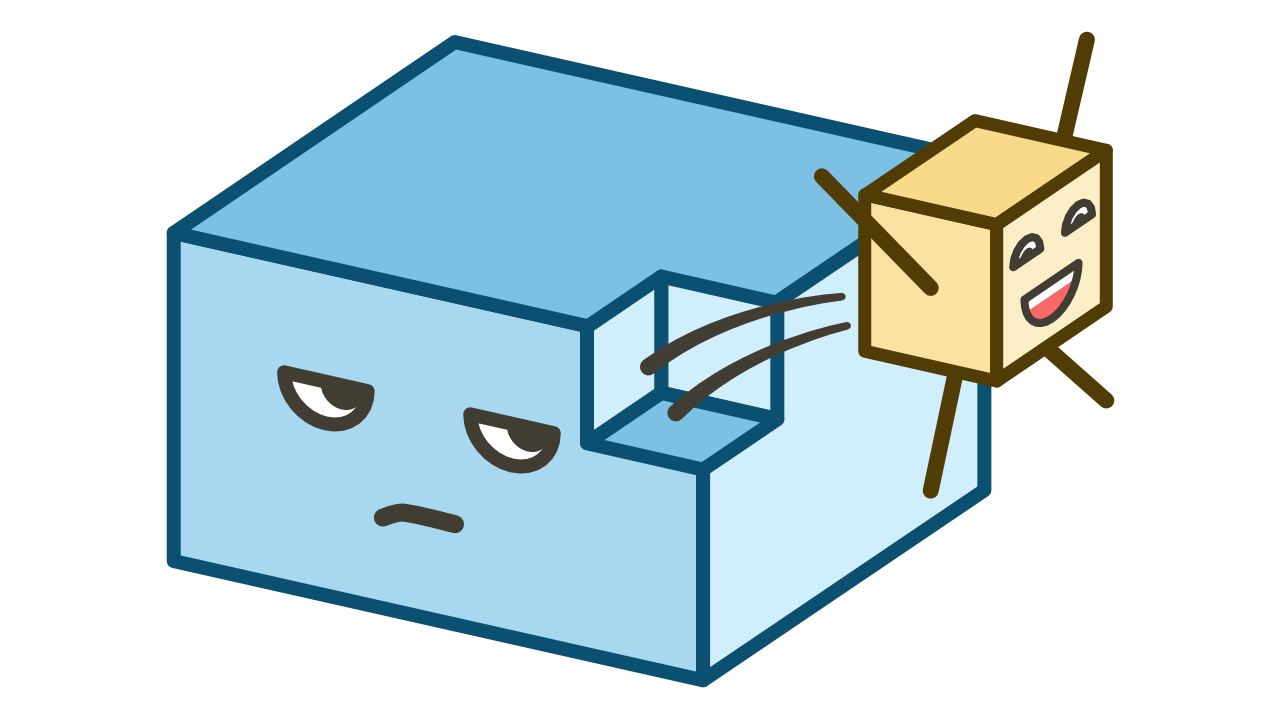
\includegraphics[width=0.4\linewidth]{assets/illustration-monolith-microservice.png}
  \label{fig:illustration-monolith-microservice}
\end{figure}


\section{What is a monolith?}

Before defining a microservice, it is advisable to understand what a monolith is since we are going to use them as a comparison. A monolithic is an "application built as a single unit" ~\cite{microservices.2014}. Enterprise applications are built with a single code base that is maintained in one place by a team or several teams, all working on that one application. Three horizontal layers often separate these applications, the data persistence layer, or database, the server, and the client. The cuts for these layers run along technological boundaries instead of boundaries related to business domains. A business domain is, for example, a part of a software that takes care of user management, another domain may be concerned with all payment-related parts of the application. A layer, however, groups all part of an application that uses the same technology, for example, Java as the server-side language.

The term "monolith" describing an extensive system derives from the Unix community, which uses the term to describe systems that became too big ~\cite{raymond.2003}. When the term is used in literature or conversation, it usually describes a system that has grown very large over time and is very unwieldy for developers to work with. The development of monolith systems tends to be slow, and maintenance is high. Such systems are widespread in the industry and usually so big that several developer teams are needed to keep them running. Because a monolith is a single unit, it is very natural for its programming code to become tightly coupled between its various modules. This has the effect that programmers need more time to understand relationships inside the code than actually writing new code. Developers do not favor large applications of this type.


\section{What is a microservice?}


\begin{itemize}
  \item \done{General definition and how it works}
  \item \done{Get some ideas from the it-innovations article ...}
\end{itemize}

A microservice has four characteristics that set it apart from a monolith.

\subsection{Independently Deployable Services}

Every software is made up of smaller parts, usually called components. The basic concept of Object-Oriented programming, for example, is that all functions and data related to one object, like a product of a store, live in one class. The class houses the data and exposes methods for other parts of the application to interface with its data. The whole application is tied together by function calls that happen inside the memory of a physical machine.

A microservice, on the other hand, is an application that lives on a physically different machine from other services and communicates through mechanisms like an HTTP request. Services don't always have to be on separate machines, but they are always treated like closed systems, and communication happens as if they were on physically separate machines.

Changes in one part of an application that consists of components only take effect when redeploying the whole application. For monoliths, this means that even small changes relative to the entire codebase require a redeploy of the whole system. A system made up of microservices only needs to redeploy the specific service where the change was made. A change in one service may also depend on a change of another service, which means there needs to be some coordination when updating them. However, in general, a microservice is independent of its neighbors and can be deployed and, more importantly, scaled as such.


\subsection{Organized around Business Capabilities}

In his excellent article about microservices ~\cite{microservices.2014} Martin Fowler mentions Conway's Law ~\cite{conway.1968} in regards to large applications. The law states that "any organization that designs a system [...] will inevitably produce a design whose structure is a copy of the organization's communication structure." An organization's structure for software projects often groups different technologies into layers, which leads to different teams skilled for different tasks. An example may be the backend team and the frontend team. Working cross team is usually accompanied by some red tape like budget approvals leading to teams optimizing to solve problems internally. This leads to business logic ending up in places of the system where it shouldn't.

There are many ideas to minimize this effect, a more popular one being Domain-Driven Design ~\cite{evans.2003}. All these approaches, however, call for discipline during development. A microserver, on the other hand, is not organized around technology but a business need. For example, the hands-on part of this paper deals with a service for generating a PDF document. A team working on a microservice, therefore, needs to be cross-functional and therefore avoids organizational barriers.


\subsection{Decentralized Governance}

When splitting an application into multiple services the developer has the choice which technology to use. Does he want to build a simple backend API and is comfortable in JavaScript, then Node.js he could use Node.js. Is he more familiar with Java, then he could set up a simple Java Spring Framework. Or maybe he needs to use some machine learning model for image processing in which case Python may be the best choice. Programmers prefer using the right tool for the right job. Monoliths have the inherent limitation that every part of it has to use the same technology. Of cource, just because it can be done doesn't mean every service has to use a different technology. Often a company is limited by the skillset present among its employees and want's to use this knowlege. Even then every team has the freedom to define their own principles and pick standards best suited for their use-case.

\begin{figure}[ht]
  \centering
  
\includegraphics[width=0.4\linewidth]{assets/illustration-monolith-hammer.png}
  \caption{Not every problem is a nail}
  \label{fig:illustration-monolith-hammer}
\end{figure}

Amazon's "You build it, you run it" methodology is a good example for the advantages of decentralized governance ~\cite{amazon.2015}. The idea is that the same team which builds a service is also responsible for running it. According to Stephen Orban, General Manager of an AWS Service, this "forces development teams to think about how their software is going to run in production as they design it." Leading to better software quality and more ownership among the team. Because they are ultimately responsible an effort is made to avoid bad practizes. According to Orban this even leads to more automation, because developers are inherently lazy and try to avoid repetitive tasks, and more customer satisfaction because the dev team has direct contact with the customer.


\subsection{Decentralized Data Management}

Decentralized data management is likely the single biggest challange with service oriented architectures. Monoliths use a single database for the entire application which makes data management easy. Microservices can also share a single database which would avoid the problem of having to save data in a distributed way or sync data across multiple databases, see figure \ref{fig:decentralised-data}. So why should microservices manage distributed data? The answer is encapsulation, which is a term in computer sience essentially saying that one component should handle all of its own concerns internally and another component should not know about them ~\cite{krivtsov.2019}.

Say there are two microservices, a user service and an order service. Each order is associated with one user who made the order. If both services have their own database then the order service saves the user ID in its database. If a request asks for an order bundled with the user information then the order service has to make a request of its own to the user service to get the user information in the first place before it can bundle it with its order and send out the answer. If the user service is not available, the order service can not finish the request. Now both services access the same database, the oder service no longer needs the user service because it can simply got into the database an get the user information itself. However, this would mean that the order service knows about the internal affairs of the user service. It know, for example, how the user table looks like. Now the two services are coupled. If a change is made to the user service the order service also has to be adjusted. This would effectively undo the benefit of using microservices in the first place and introduce all the challanges of large monoliths into the service oriented architecture.

\begin{figure}[ht]
  \centering
  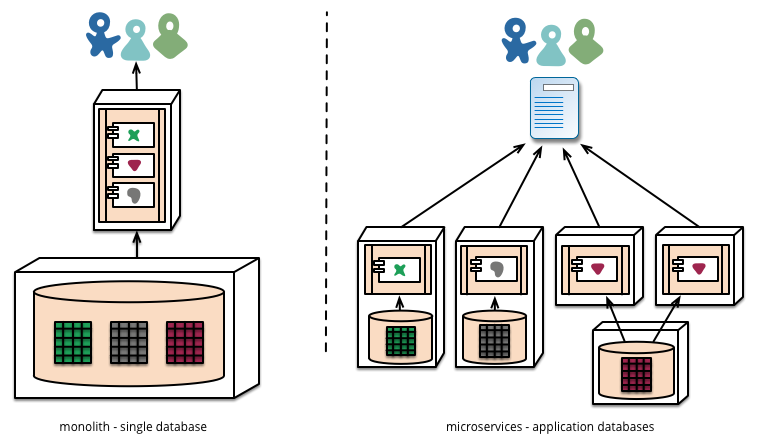
\includegraphics[width=0.7\linewidth]{assets/decentralised-data.png}
  \caption{Data management of monoliths and microservices}
  \source{https://www.martinfowler.com/articles/microservices.html}
  \label{fig:decentralised-data}
\end{figure}

Decentralized data management is the main reason why microservice architecures are not the golden bullet solution. Even though the benefits of microservices outweigh a monolith architecture in the long run, there is a consensus among developers that it is better to start with a monolith and refactor to microservices "if you really need them in future." ~\cite{krivtsov.2019}


\section{Why are microservices currently interesting?}

\begin{itemize}
  \item \todo{(Why)}
  \item \todo{Application development until now with monoliths \& waterfall}
  \item \todo{Avarage life and maintenance effort of a big application}
  \item \todo{Rise of Agile, the Cloud and quick deployment cycles}
\end{itemize}


\section{Which problem does a microservice solve?}
\label{sec:theory:what-problem}

\begin{itemize}
  \item \todo{(Why)}
  \item \todo{Why is a microservice better than a monolith?}
  \item \todo{Advantages \& Disadvantages of microservices}
  \item \todo{Work/Effort of microservice compared to monolith}
\end{itemize}


\section{When does a microservice make sense?}

\begin{itemize}
  \item \todo{(Why)}
  \item \todo{What type of application are microservices best suited for? (Scallable, defined scope)}
  \item \todo{Good size of a team for a microservice}
  \item \todo{When not to use distributed service architecture}
\end{itemize}


\section{How to extract a microservice?}

\begin{itemize}
  \item \todo{(How)}
  \item \todo{How to make a cut in a big application (monolith)}
\end{itemize}


\section{Challenges of implementing a microservice}

\begin{itemize}
  \item \todo{Complexity of ecosystem}
  \item \todo{Design challange because often monolith software is old and overcomplicated. This complication should be simplified in the new microservice.}
\end{itemize}

\chapter{CEMicro Architecture and Technology Stack}
\label{sec:arch}

This chapter takes us through the journey of planning and designing the CEMicro service. We understand the boundaries and features of the so-called ``Configurable Elements'' of the POS application and learn the goals Capgemini has with this project. Several times initial assumptions about the final service are challenged, and new and better design decisions made. We also decide, or sometimes somewhat justify, the technology decisions for the later implementation of CEMicro.

\begin{figure}[ht]
  \centering
  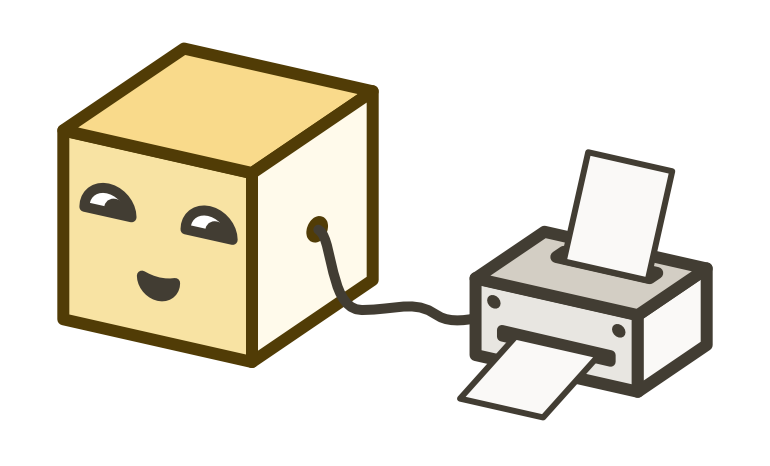
\includegraphics[width=0.4\linewidth]{assets/illustration-microservice-printer.png}
  \caption{CEMicro is responsible for the ``Configurable Elements'' of printed documents}
\end{figure}

\section{The existing appliction}

The existing application which this department of Capgemini is working on in a point of sales (POS) software. It is essentially the toolkit a salesman uses to create an offer for a potential customer. Since cars are a highly configurable product, the POS software has to support a wide variety of options. It is made even more complicated by the different types of cars, different types of brands, or sub-brands, and the fact that it is in use across several markets and languages. Each market has its very own requirements and levels of hierarchy, which the application reflects in terms of user management and access levels.

The part of the application which involved my task is the creation of the final offer as a printable PDF document. Depending on the object of the sale, the type of car, the current market, and a host of other factors, the application will decide which document template to use. It will then collect the appropriate lines of text and values from the database to assemble into a finished document, which it then generates in the PDF format. Additionally, there are several configuration pages in the admin area of the application that manages these templates and defines their contents. Figure \ref{fig:pos} shows a glimpse of the somewhat unwieldy admin interface for the part of the document creation.

There are currently nine teams of about six developers, each working on the POS application.

\begin{figure}
  \begin{subfigure}[b]{0.5\linewidth}
    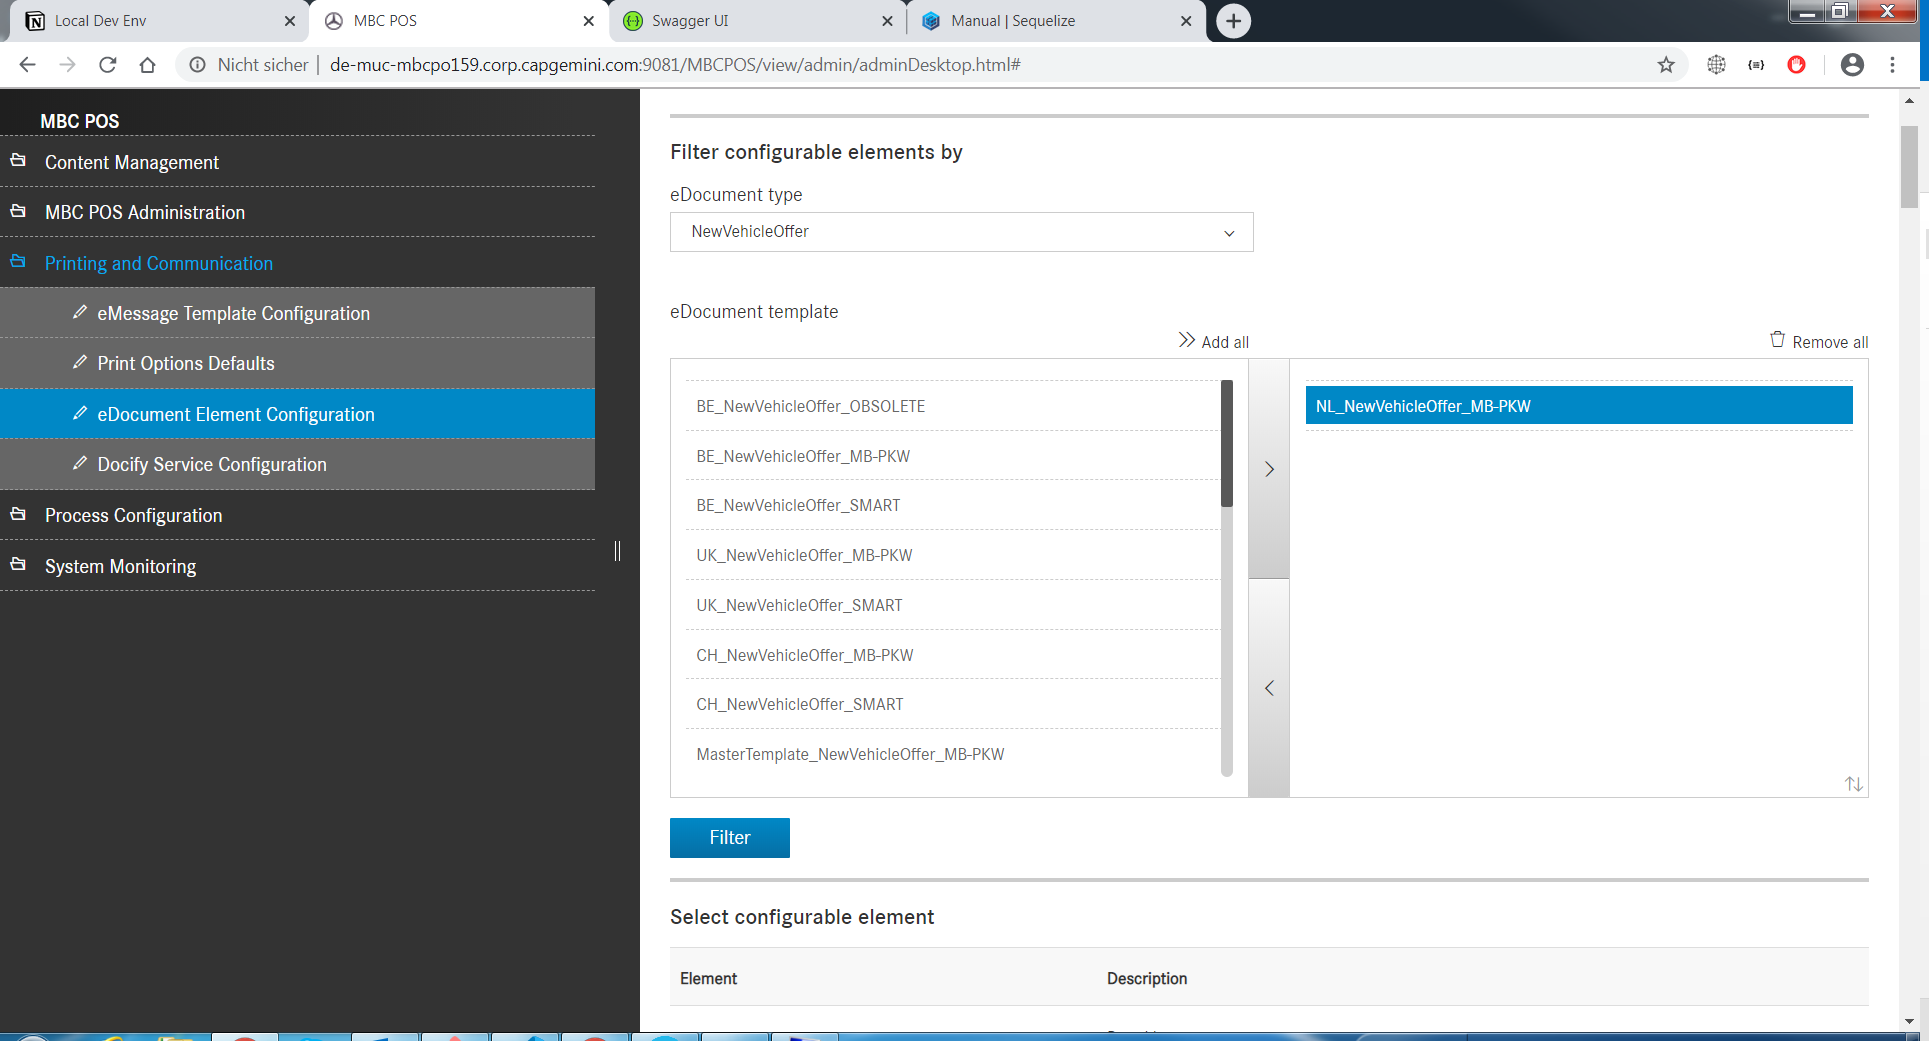
\includegraphics[width=\linewidth]{assets/pos-ce-config-1.png}
    \caption{Template selection}
    \label{fig:pos:a}
  \end{subfigure}
  \begin{subfigure}[b]{0.5\linewidth}
    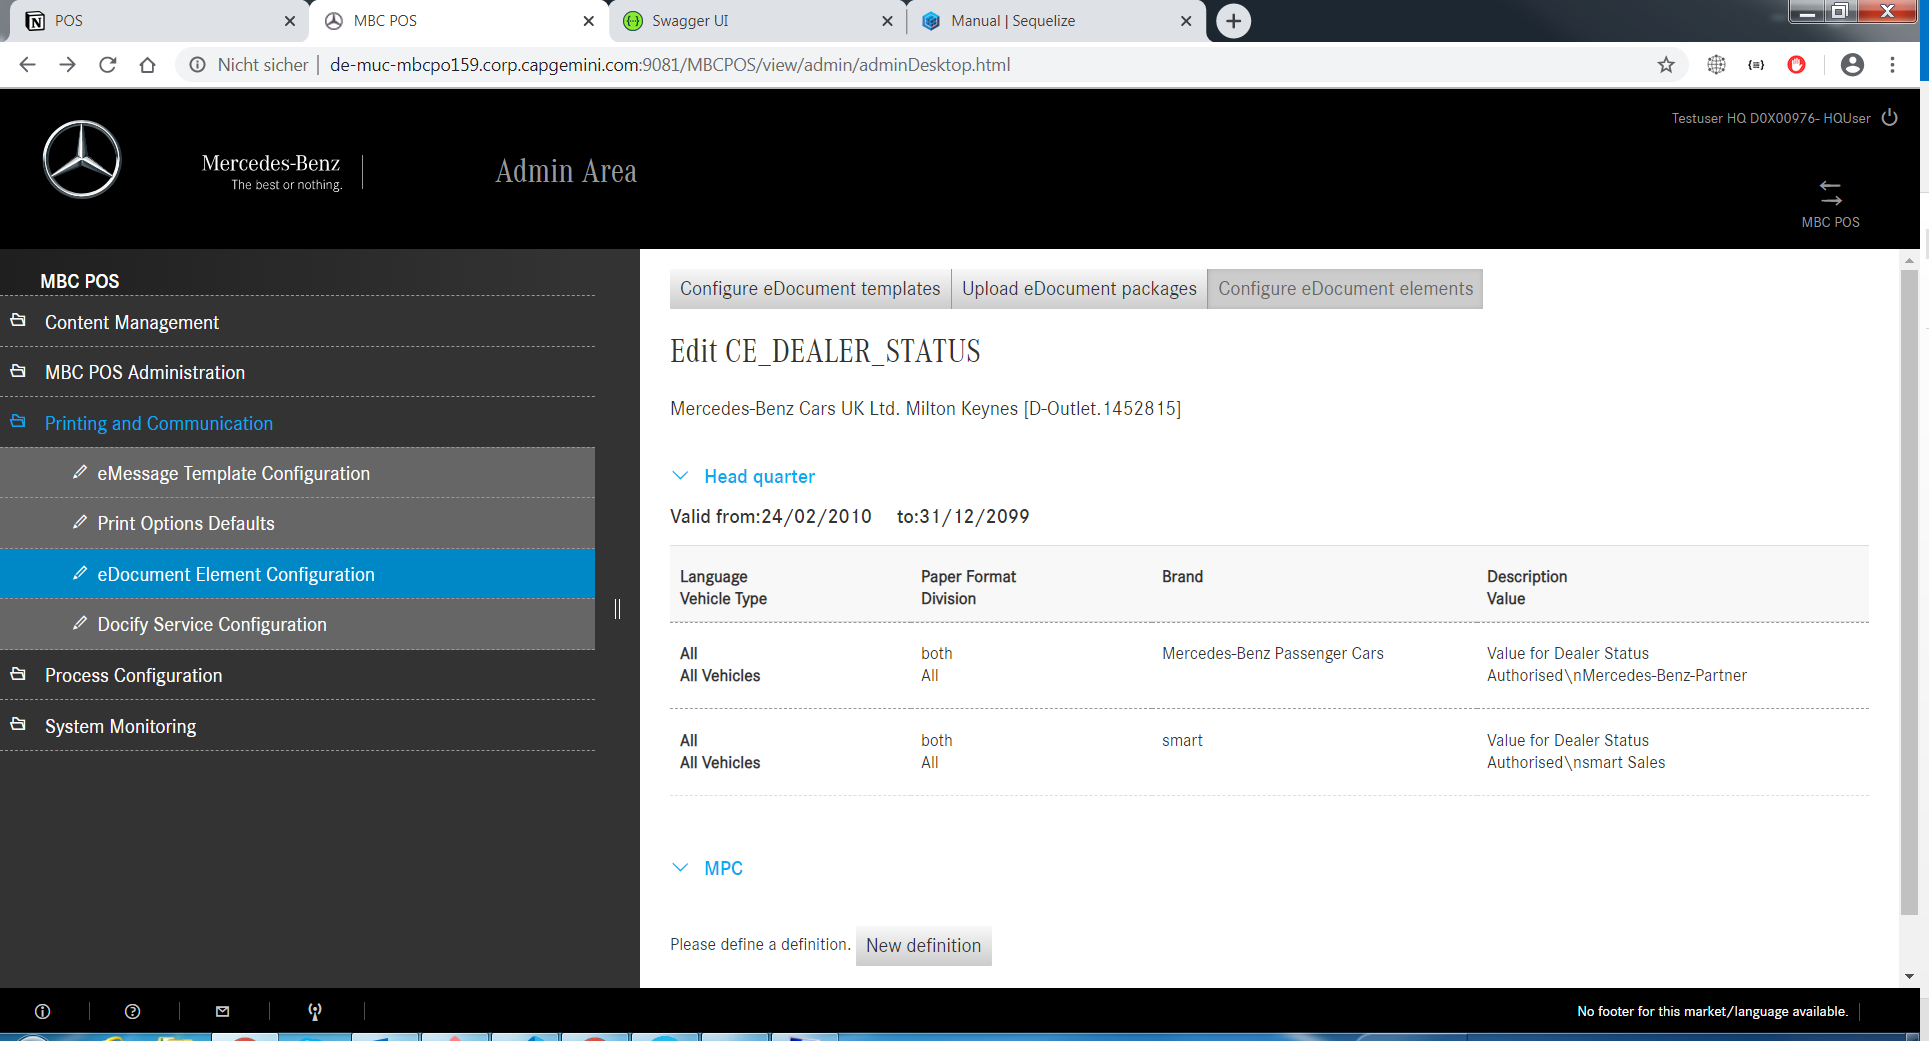
\includegraphics[width=\linewidth]{assets/pos-ce-config-3.png}
    \caption{One CE contains several children}
    \label{fig:pos:b}
  \end{subfigure}
  \caption{POS configurable element admin page}
  \label{fig:pos}
\end{figure}

The part of the application responsible for generating a printable document has been part of a past student project very similar to my task. The team of students essentially built a microservice that is responsible for managing the templates. An application programming interface (API) provides access to the service and returns the finished PDF. They called this service Docify.

Docify is a kind of textbook example for a microservice. A document printing service lends itself very nicely to be extracted into its separate application because its interface is so clearly defined. The interface for a printing service requires two properties, first, the name or identifier of the predefined template, and second, the dataset which is needed to fill the gaps of the template. That often means the biggest challenge for distributed services, defining the boundaries, and thus their interfaces are no-brainers for this use-case.

Figure \ref{fig:docify} shows the administration interface for Docify, and it is easy to see how each of the two previously mentioned API criteria has its page. On the left \ref{fig:docify:a} is the list of templates, the identifier of each template is a client-market-name tuple, and on the right \ref{fig:docify:b} is the editor for template specific templates with the HTML representation on the left and the rendered preview. The HTML code contains several placeholders which replace their respective value when printing document.

\begin{figure}
  \begin{subfigure}[b]{0.5\linewidth}
    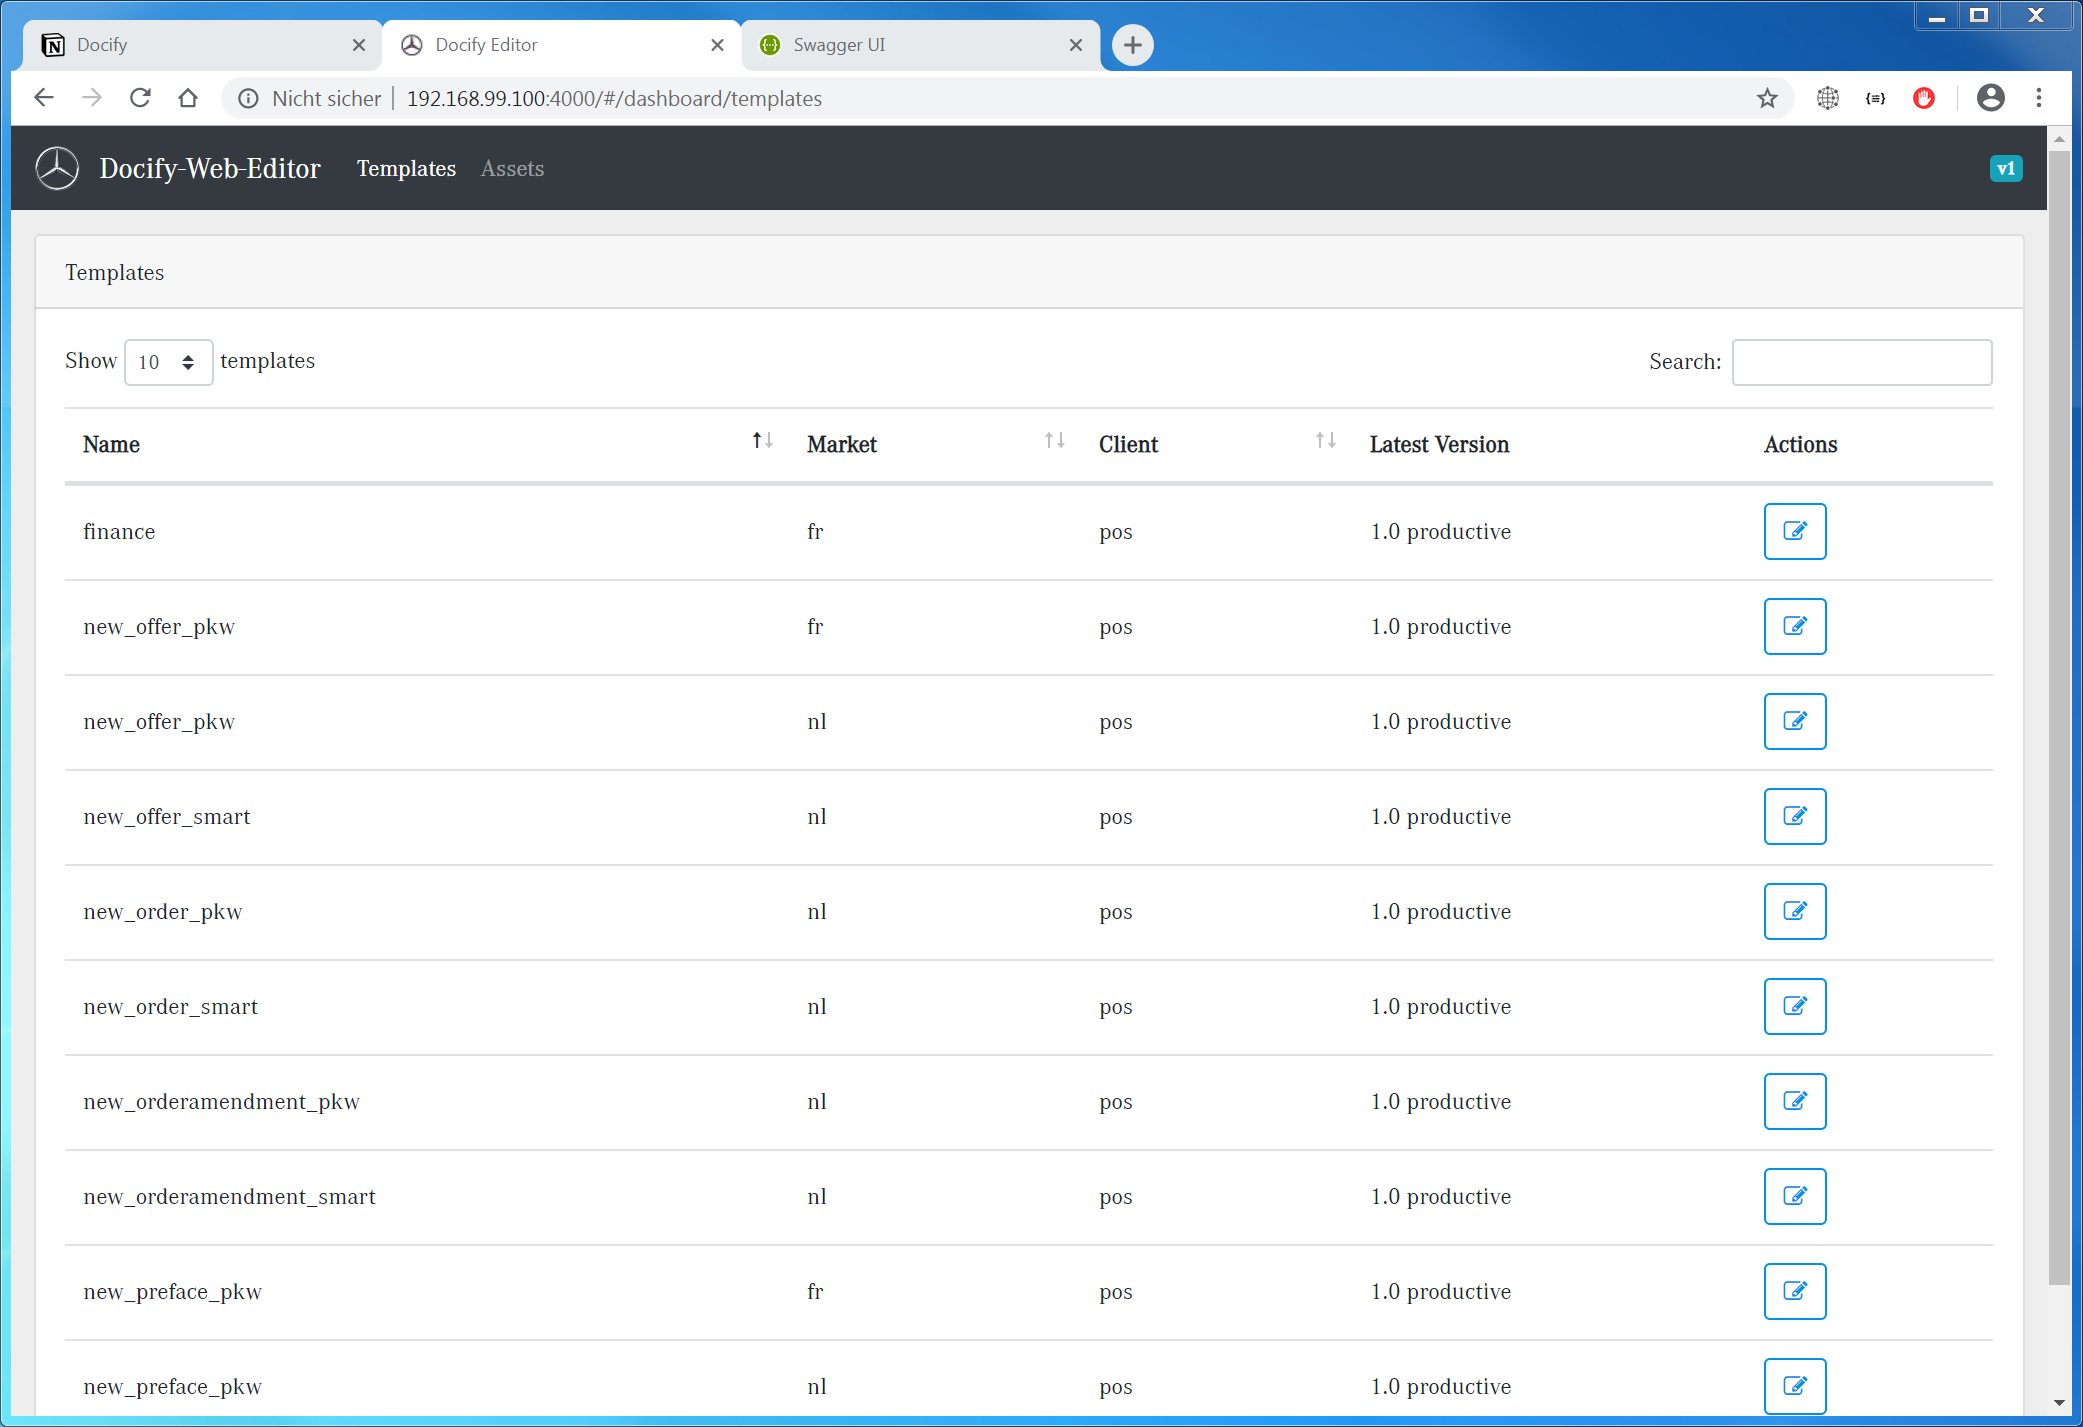
\includegraphics[width=\linewidth]{assets/docify-template-list.png}
    \caption{Template list}
    \label{fig:docify:a}
  \end{subfigure}
  \begin{subfigure}[b]{0.5\linewidth}
    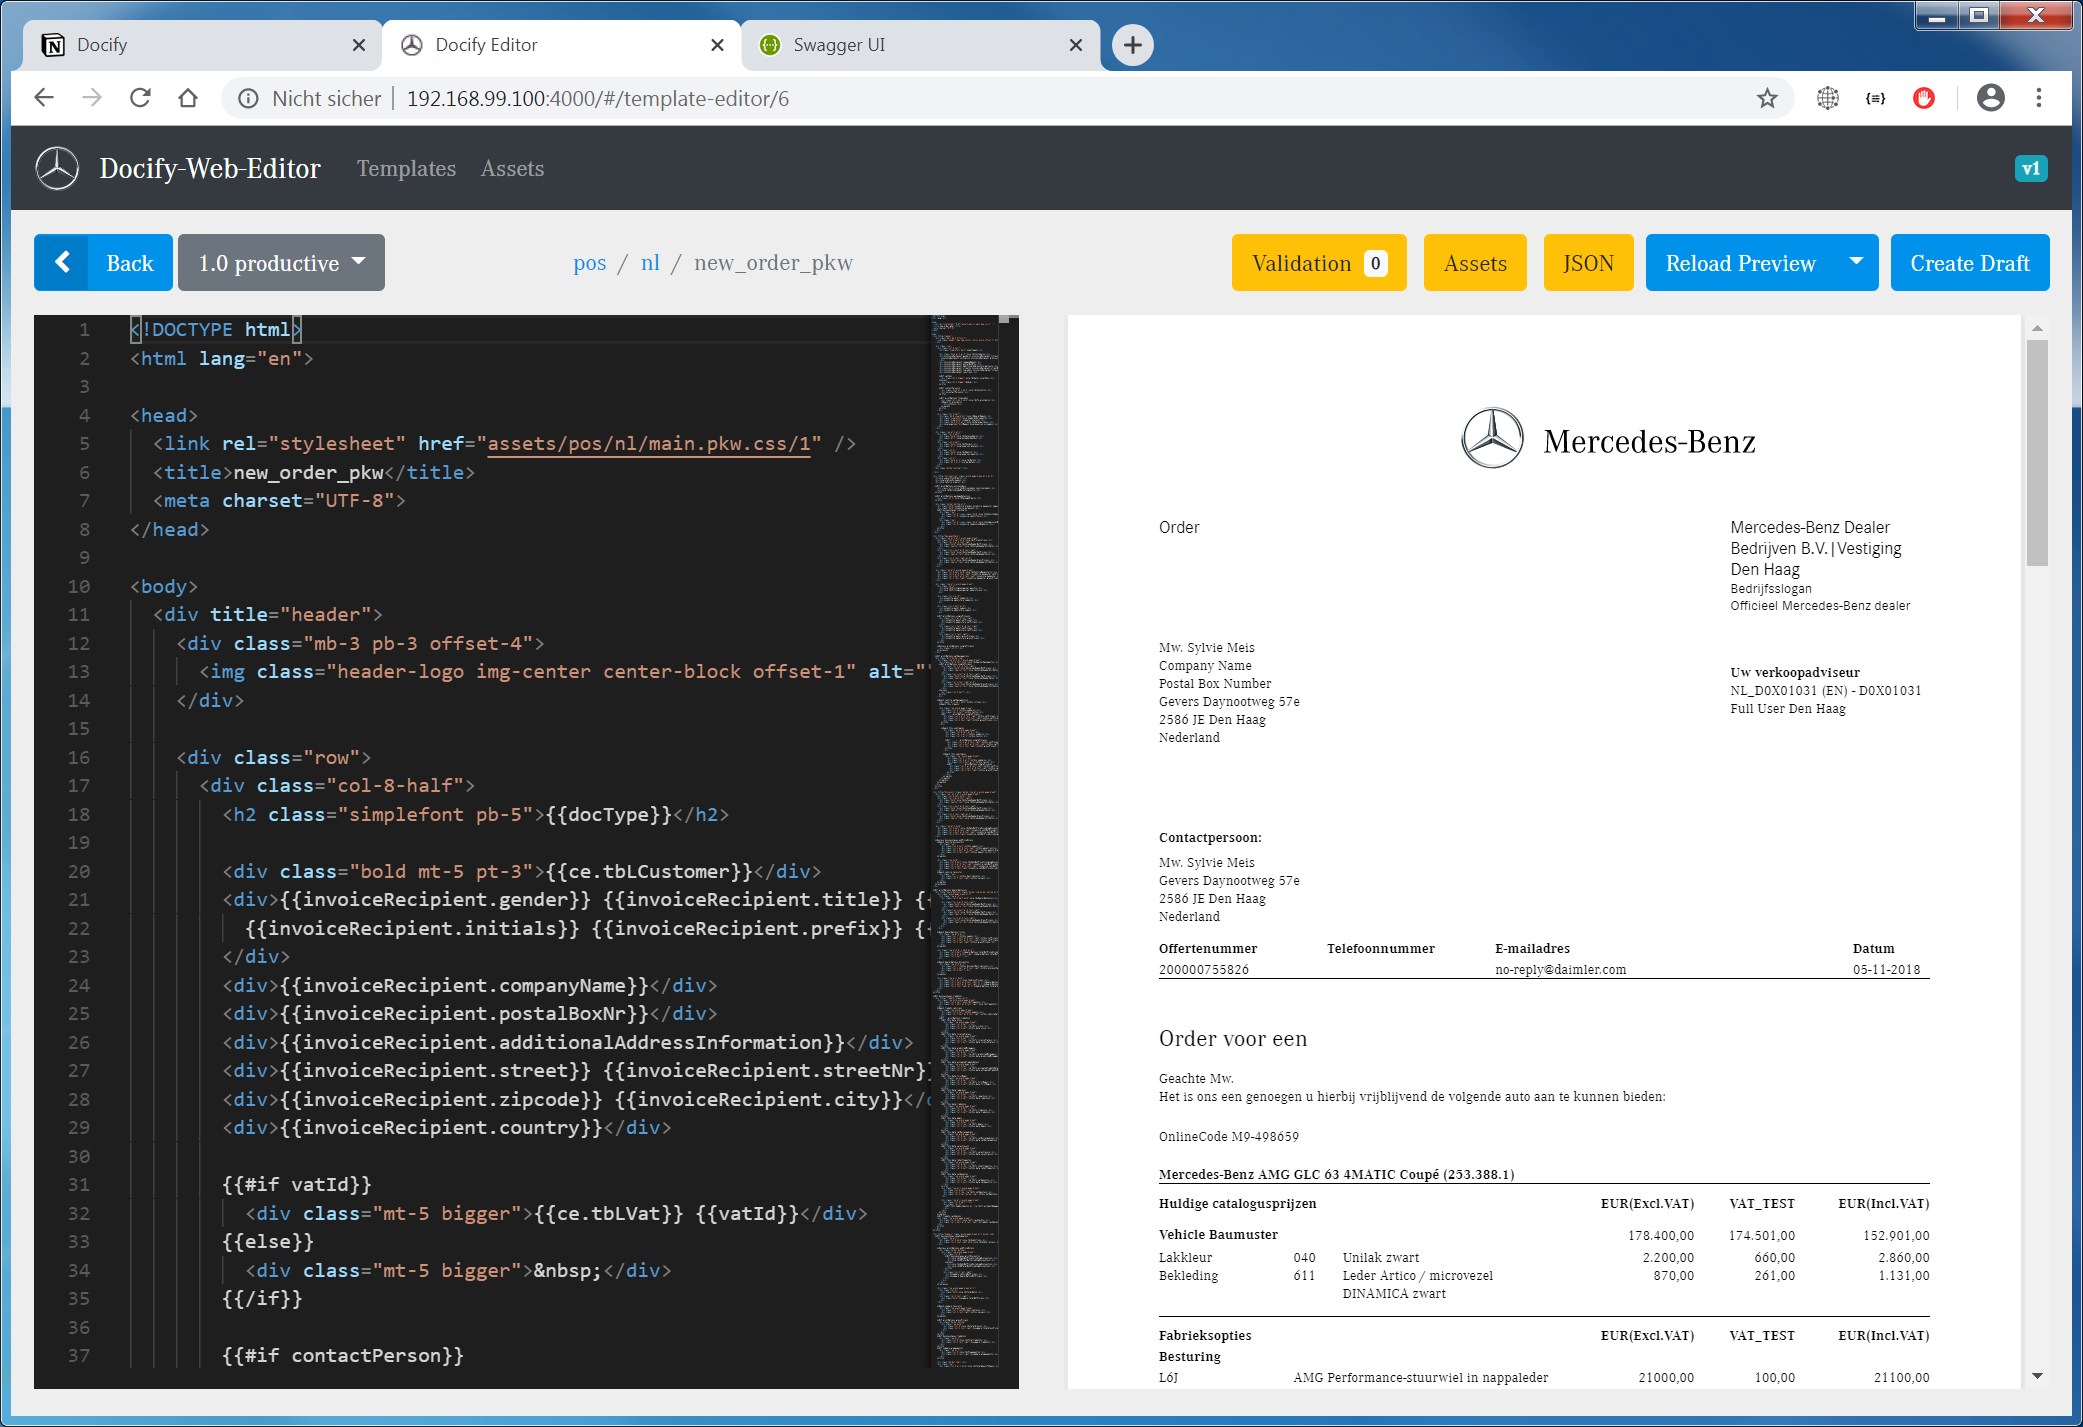
\includegraphics[width=\linewidth]{assets/docify-editor.png}
    \caption{Template editor}
    \label{fig:docify:b}
  \end{subfigure}
  \caption{Docify template editor app}
  \label{fig:docify}
\end{figure}

While the technical aspect of Docify might be simple, it is interesting to observe the non-technical challenges that a microservice is facing. Besides the question of how a microservice should be extracted and build, there is the economic question of why it is necessary to invest the time into creating such a service when it seems to be working just fine as it is. The question every project has to face is, ``Does it add business value?'' and if it doesn't, why should the business spend money on the project? This is an interesting question especially for engineers who often try to build the ideal solution for a problem, after all, that's why we became engineers in the first place, but forget that our time is valuable and to build the ideal solution, in this case, a microservice, for an already working feature may not make much sense to the business as a whole.

So why was Docify build in the first place? I haven't been involved myself, but from the proceedings with my project, I can surmise some good indicators. On the one hand, the POS application is over five years old, which in the world of software is a man with a cane and a white beard. Over the lifetime of any software, it tends to become ever more complex and both in its technical scope but also in terms of management. Thus even small changes to the codebase can take several days or even weeks until the task gets prioritized, implemented, and deployed. In the ideal situation, the database contains all the parts which users are supposed to be able to edit so that changes don't have to be handed to developers, but in the case of POS, many adjustments to the document creation could only be made by direct manipulation of the codebase which meant that a task hat to be created for developers.

One example of this directly involves my task, the so-called ``Configurable Elements,'' which I will describe in more detail in the next section, are basically texts that can be edited by users. But the definition for these elements is hardcoded in the application, meaning if users want to add a new such item, they have to create a task for devs to do so, which adds considerable friction to something which should be just one click. Essentially, Docify enables users to do administrative tasks directly while saving all the development time of adding these admin interface features to the existing monolith codebase.

The other business value has to do with the fact that there is currently a particular hype around microservice architectures. The project of Docify enabled Capgemini to showcase this architectural model on a reasonably simple use-case to its client while not losing much in terms of wasted development time if the client declines its further development. And since a microservice can be built in a completely separate tech stack, it was mostly a proof of concept/demo of a flashy new architecture and some flashy new technology.

In the end, the client liked what business value Docify had to offer and was willing to invest in its development. At the time of this writing, Docify is two years old and was rolled out to two of the several markets POS is operating in. Meaning even after two years of development, the POS team is still maintaining the old implementation in spite of the new and shiny microservice, which is probably an appropriate image of how large companies tend to operate if their internal structures became sufficiently complex.


\section{Goals of the CEMicro Service}

\begin{itemize}
  \item \done{What is the microservice supposed to do}
  \item \done{High-Level Overview of Illustration}
  \item \done{The complexity of POS / CE Properties}
  \item \done{Out of scope: Access control}
\end{itemize}


As already noted in the previous segment, the idea of a microservice for document creation is pretty straightforward since the API is well defined from the get-go. The printable document handling in POS, however, has three parts. Besides template and dynamic values, which are different on a per offer basis, it defines a number of static values inside the templates, which are called ``configurable elements.'' The idea behind configurable values, or CEs in short, is, that they are the same on every printout, but can be defined according to a number of factors like the current language if the paper is branded or blank if a new or used car is sold and so on.

The next segment will go into more detail what complexity was actually hidden behind the rather primitive looking CEs but suffice to say at this point, the setting of these static values for a printable template is cumbersome and complicated by nature.

My task, therefore, was to extract the configuration of these CE values into a separate service, which can be queried by the POS system to retrieve the correct set of CE values for any given document template under a given set of conditions. For example, if the salesman using POS wants to print an offer for a new car in the Netherlands on blank paper, the POS application would then send a request to this new service saying: ``please give me all the configurable elements I need to print a new offer for this and that car in the Netherlands marked on blank paper.'' The responsibility of the service would then be to produce a list of key-value pairs that the POS application can then hand to the Docify service, or its internal printing function for that matter, to be inserted into the configurable element placeholders in the document template.

Not much guidance was given to me beyond this point from Capgemini. I was given access to the source code of both the POS application and the Docify service and could start them on personal virtual machines to understand their working. Because several teams of developers were working on POS and after seeing the size of the codebase, I quickly concluded that it would not make much sense for me to try to understand the inner workings of the existing Java code. Instead, I decided to investigate the user interface of both services, and in the case of Docify, the API to understand what features my service needs to offer and what interfaces it should expose.

I decided to call the service CEMicro, short for Configurable Element Microservice. The name is rather dull and not in the vain of more modern hipster names like Spotify or Instagram, but it serves a very functional purpose in quickly communicating what it is supposed to do to an audience that is familiar with the existing cumbersome feature of configurable elements. I felt choosing a functional name that eases the adoption of a new service was more expedient than a beautiful and fancy name.

Early in the planning of the application context, that is, with whom the new application needs to communicate about what, I assumed that CEMicro only needs to talk to the POS system since, in the end, only the POS system will request a dataset from CEMicro. But after understanding that the templates are actually not available to POS but rather maintained by Docify, it became clear to me that either CEMicro has to have its own copy of each template or it needs to request the template from Docify in order to know which configurable elements the template requires. Another option would have been for users to tell CEMicro which configurable elements exist and are part of which template, but this would have meant a double effort for users since each new CE that was defined inside a template in Docify needs to be additionally added to CEMicro, which brings us to the concept of the single source of truth.

The single source of truth [ref] is a fundamental concept in programming that value or variable should only be defined and maintained in one place, the source of truth. As soon as they are set in multiple locations, there has to be a system to keep each other synchronized; otherwise, the application state will be inconsistent. The single source of truth principle thus becomes even more critical for a distributed service architecture. In a monolith application, and this is really the reason why monoliths are more comfortable to develop and more widely used, there is usually only one database, and the whole application has access to all the data. But in a distributed service architecture, every individual service only has its own database. In order to make this work, each service can only handle the data of its particular domain and has to request the data of other services through their public interfaces. In the case of CEMicro, the database can only contain the data of the actual configurable elements and not the data of the templates, or the user table for that matter. If copies of a dataset existed in the databases of multiple services, there would need to be a mechanism to keep all these copies in sync. This can be done through a publish-subscriber pattern [ref], but if the availability of the network can not be guaranteed, and the first rule of a network is that its availability can not be guaranteed, then the data can become inconsistent between copies. And with computer systems where millions of daily requests are no rarity, the rule that what can happen will happen is pretty much a given.

It was therefore decided to include both POS and Docify in the new services context. If a user wants to manage the configurable elements of a template CEMicro will request the list of available template and then the individual template from Docify, scan it for all the placeholders which will be replaced with CE values and add a database entry for each value with a unique composite index that is comprised of the template name and the market. The user can then edit each individual configurable element, which is directly persisted in CEMicro's own database. POS can then request the list of configurable element values by the unique template name and market pair. Figure \ref{fig:context} shows the public interfaces of the CEMicro service, its related third-party applications, and its own three-layer structure of a database, server, and client.

\begin{figure}
  \centering
  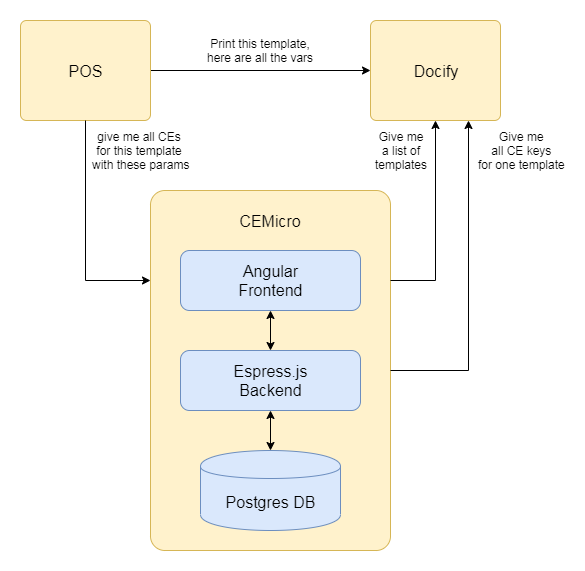
\includegraphics[width=0.6\linewidth]{assets/high-level-overview.png}
  \caption{High level context overview for the microservice}
  \label{fig:context}
\end{figure}

While the CEMicro service would become more complicated than at first anticipated, it was also decided to exclude some functionality from it. The reason is simply the limited time of the project, four months, and the nature of it being a proof of concept rather than a production-ready application.

One feature that was decided as out of scope for this project is user management or access control. The POS application has a relatively complex structure of access control with its various layers of authority, starting from the so-called HQ, the highest entity per market, through multiple levels of smaller and smaller organizational structures down to the local reseller. Each of these levels can define their own set of configuration options, which may or may not be overwritten by the next lower level of management. Because access control, especially such an elaborate one, adds another dimension of complexity to every project, it was decided to create this proof of concept without any, meaning there will only be one user who can do everything.

Another vital part of an application that was neglected is testing, both unit, and integration testing. Testing is more if an implementation detail and will, therefore, be further discussed in chapter \ref{sec:impl}.


\section{Understanding the existing feature}
\label{sec:arch:understanding}

\begin{itemize}
  \item \done{What is a configurable element?}
  \item \done{What properties does a CE have?}
  \item \done{Challenge: Understanding the task}
  \item \done{Challange/Example: Devs didn't know that CEs are not unique per template}
\end{itemize}

After defining what the microservice needs to accomplish and in what context it lives comes the next step in accurately understanding what functionality the new microservice needs to offer. Since we are extracting a microservice from an existing application, we are also extracting a specific feature set that users have been using and are used to.

Every application is faced with the question of how to expose data to the user and how to design a system's controls. In software development, this is usually called the user interface (UI) and user experience (UX). The ultimate goal is for the user interface to be intuitive to explain itself, but in any way, the user has to learn how to use the application. Even if the UI is terrible or even broken, the user will eventually learn how to use that system, even if he needs to use unintended detours to reach his goal. Once the user has determined the UI, every change will require him to re-learn even if the change is a fix of broken behavior.

An excellent example of this is Windows 8, where Microsoft decided to change the user interface of the start menu button. Every windows user has learned that the Windows Desktop is their default view, and the start menu serves as a hallway to all their applications and settings. As seen in figure \ref{fig:win8}, the start menu was removed in Windows 8 in favor of a hot corner that would lead to the new tiles interface. Even if the new interface would have been objectively better, with this decision, Microsoft asked every Windows user to re-learn one of the core concepts of its user interface. Not surprisingly, there was a huge outcry, and Microsoft quickly issues a patch with Windows 8.1 restoring the start menu the people were used to.

\begin{figure}
  \begin{subfigure}[b]{0.5\linewidth}
    
\includegraphics[width=\linewidth]{assets/windows-8-taskbar.png}
    \caption{Windows 8 taskbar without start menu button}
  \end{subfigure}
  \begin{subfigure}[b]{0.5\linewidth}
    
\includegraphics[width=\linewidth]{assets/windows-8-hot-corner.jpg}
    \caption{Windows 8 new hot corner}
  \end{subfigure}
  \caption{Windows 8 start menu UI change}
  \source{https://www.howtogeek.com/107662/how-to-live-without-the-start-button-in-windows-8/}
  \label{fig:win8}
\end{figure}

It is, therefore, imperative when extracting a microservice to understand precisely how the affected features were used by the existing users who will have to adapt to, or reject for that matter, the new service. Since I was not given a list of requirements or any sort of guideline about the precise workings of configurable elements, I took some time to understand the existing user interface and map out what kind of configurations are available to the user. The admin section for configurable element has three list view, figure \ref{fig:pos:a} shows the list of templates, figure \ref{fig:pos:c} the list of available CEs inside the selected template and figure \ref{fig:pos:b} shows a list of values that can be assigned to each CE grouped by hierarchy levels (Headquarter, MPC, etc.) and equipped witch a number of qualifying properties.

\begin{figure}
  \centering
  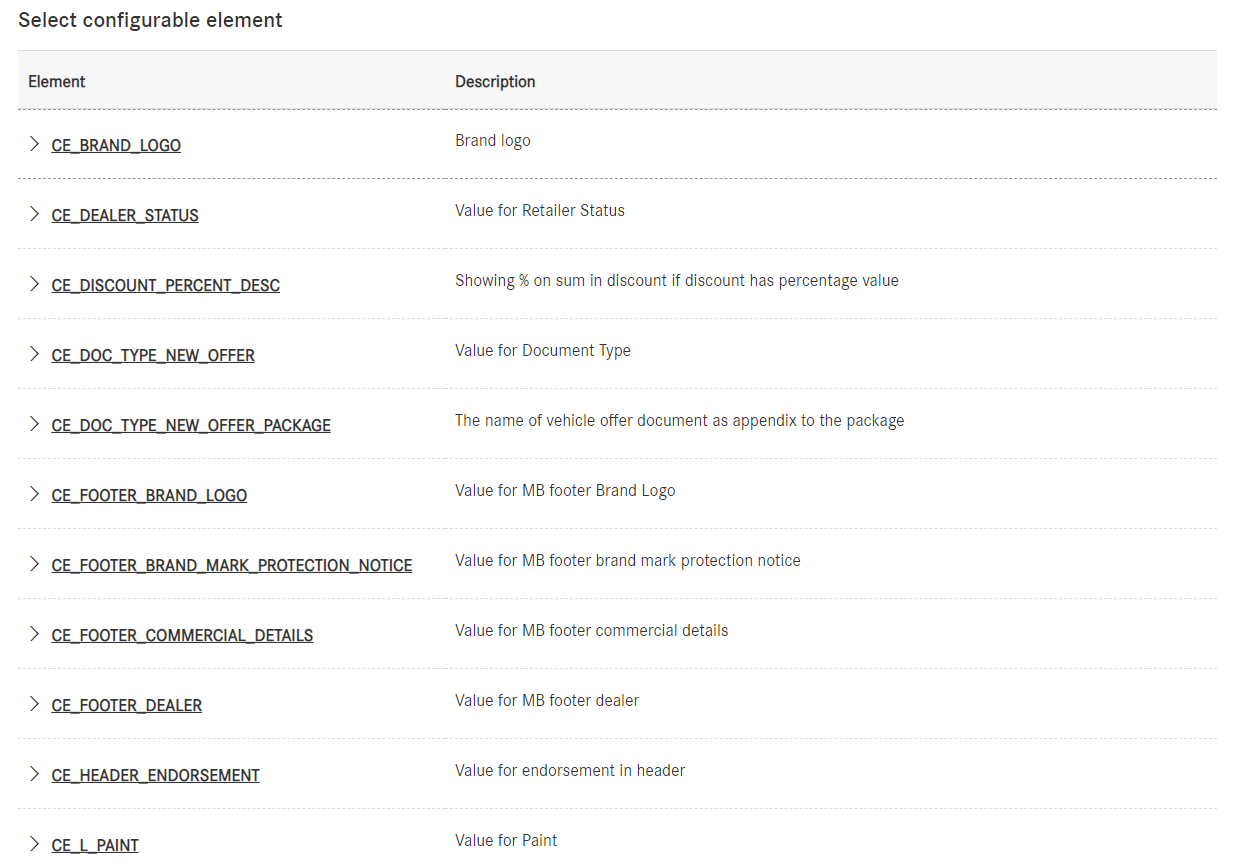
\includegraphics[width=0.75\linewidth]{assets/pos-ce-config-2.png}
  \caption{List of CE pertaining to a template}
  \label{fig:pos:c}
\end{figure}

This means CEs are not, as initially assumes, a simple key-value data structure but, in fact, can contain many values, each coming with a number of properties. These properties are later used to determine which value is the best fit for the current use case. Through testing, the possible values for each property were identified and mapped out in table \ref{table:ce-properties}. Figure \ref{fig:ce-properties} shows how these properties are presented to the user. Note how it is not immediately apparent that the valid from-to dates are part of the configuration and that they can, in fact, be changed. Also note the confusing layout of the value and description text inputs, the description which has no real purpose being the first input while the actual value of the configurable element, the most important thing of the whole interface, is the last input field of them all. Additionally, website users are more used to ``value'' fields being a single line and ``description'' fields being multi-line, here this logic is inverted.

\begin{table}[!ht]
  \begin{center}
    \begin{tabular}{|l|c|p{10cm}|}
      \hline
      Property & Required & Possible Values \\
      \hline\hline
      Name & * & [any] \\
      \hline
      Value & * & [any] \\
      \hline
      Description & & [any] \\
      \hline
      Language & & Any Language, English, German, French, ... \\
      \hline
      Paper Format & & Branded, Unbranded \\
      \hline
      Valid from-to & & [dates] \\
      \hline
      Vehicle type & & New Vehicle, Used Vehicle, Both \\
      \hline
      Division & & Any, MB Passenger Car, MB Van, Foreign Brand Passanger Car, MB Passenger Car \\
      \hline
      Brand & & Any, Mercedes Benz Passanger Cars, smart, Mercedes Benz, OTHER \\
      \hline
    \end{tabular}
  \end{center}
  \caption{Possible properties for configurable elements}
  \label{table:ce-properties}
\end{table}

\begin{figure}
  \centering
  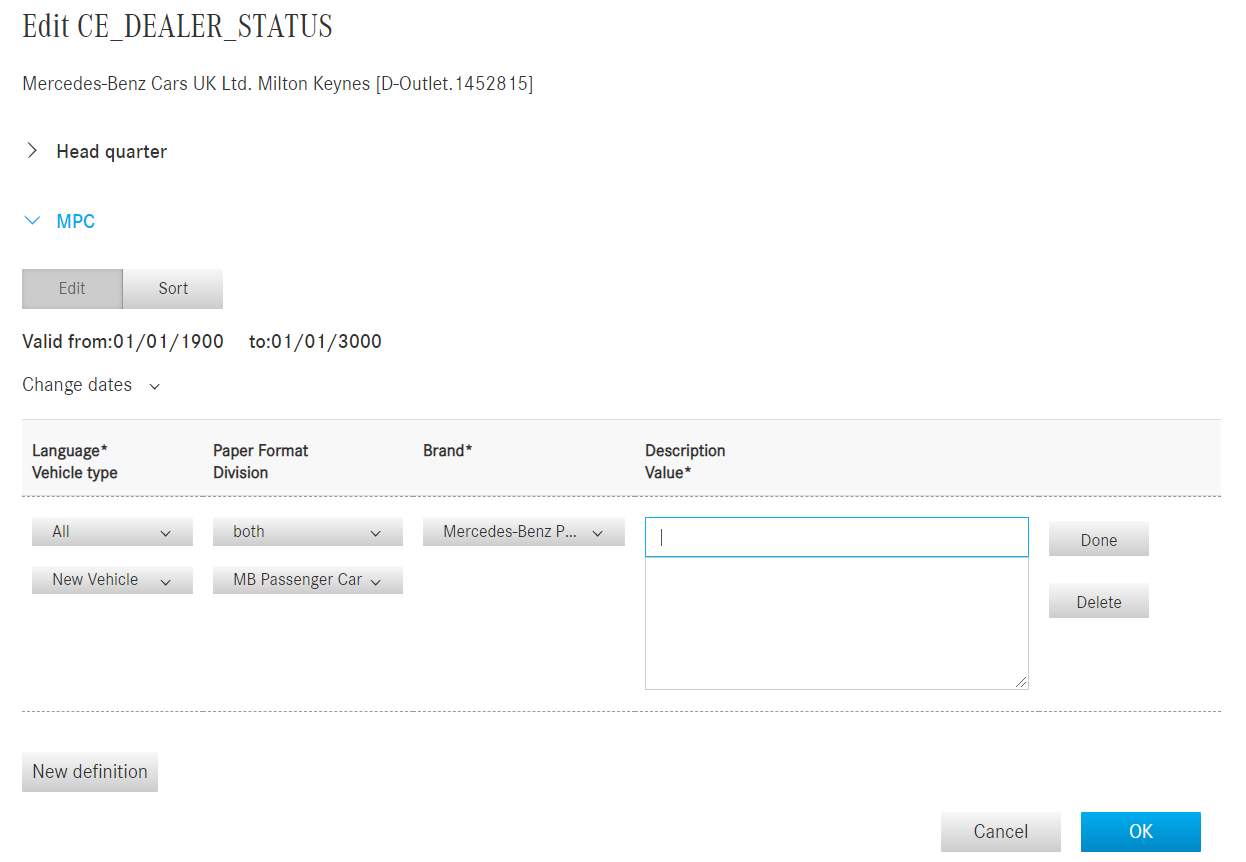
\includegraphics[width=0.8\linewidth]{assets/pos-ce-config-4.png}
  \caption{Configurable element configuration properties}
  \label{fig:ce-properties}
\end{figure}

The challenge of this task was, as already noted that no definite list of requirements or guidelines existed for the configurable elements feature, which should be extracted as a microservice. An intriguing detail showcasing this was my advisor's surprise when I told him that configurable element names are not treated as unique per templates, meaning if multiple templates contained CEs of the same name and the user would change the value of one, then the change was reflected for the other templates as well. I asked him if this was intended behavior, and he answered that he had always assumed the values to be unique to each template. I, therefore, decided to namespace the CEs with their respective market-templates tuple in the CEMicro application as this behavior was more intuitively expected.

Now that I had a comprehensive understanding of the current feature set for configurable elements, I could start drafting the user interface and application programming interface of the new CEMicro service.


\section{Deciding the Technology}
\label{sec:arch:technology}

I decided to build CEMicro as a modern web app. A web app is a website that behaves like an application instead of merely showing information to the user. It consists of three layers, as shown in the context diagram in figure \ref{fig:context}. The client is the user interface that the browser displays, the server provides the API and business logic for the client and the database to store the data.

The client is made up of a markup language HTML for the browser together with CSS for visual styling and a templating engine pr frontend framework written in JavaScript. Javascript is a programming language that can run natively inside every browser. There are other languages a browser can run like Java, but only with appropriate plugins. While browser vendors first introduced JavaScript in the early days of the internet with the very first Netscape and Internet Explorer browsers, it has only become a viable choice for more ambitious projects during the last decade\footnote{I am writing this in 2020}. Only then the language became versatile enough and especially gained sufficient browser support to be considered for more significant projects. An excellent example of this is so-called promises, a data type needed for asynchronous programming, which both Chrome and Firefox only support since 2014 ~\cite{caniuse.2020} as seen on the graph in figure \ref{fig:caniuse-promises}.

\begin{figure}[ht]
  \centering
  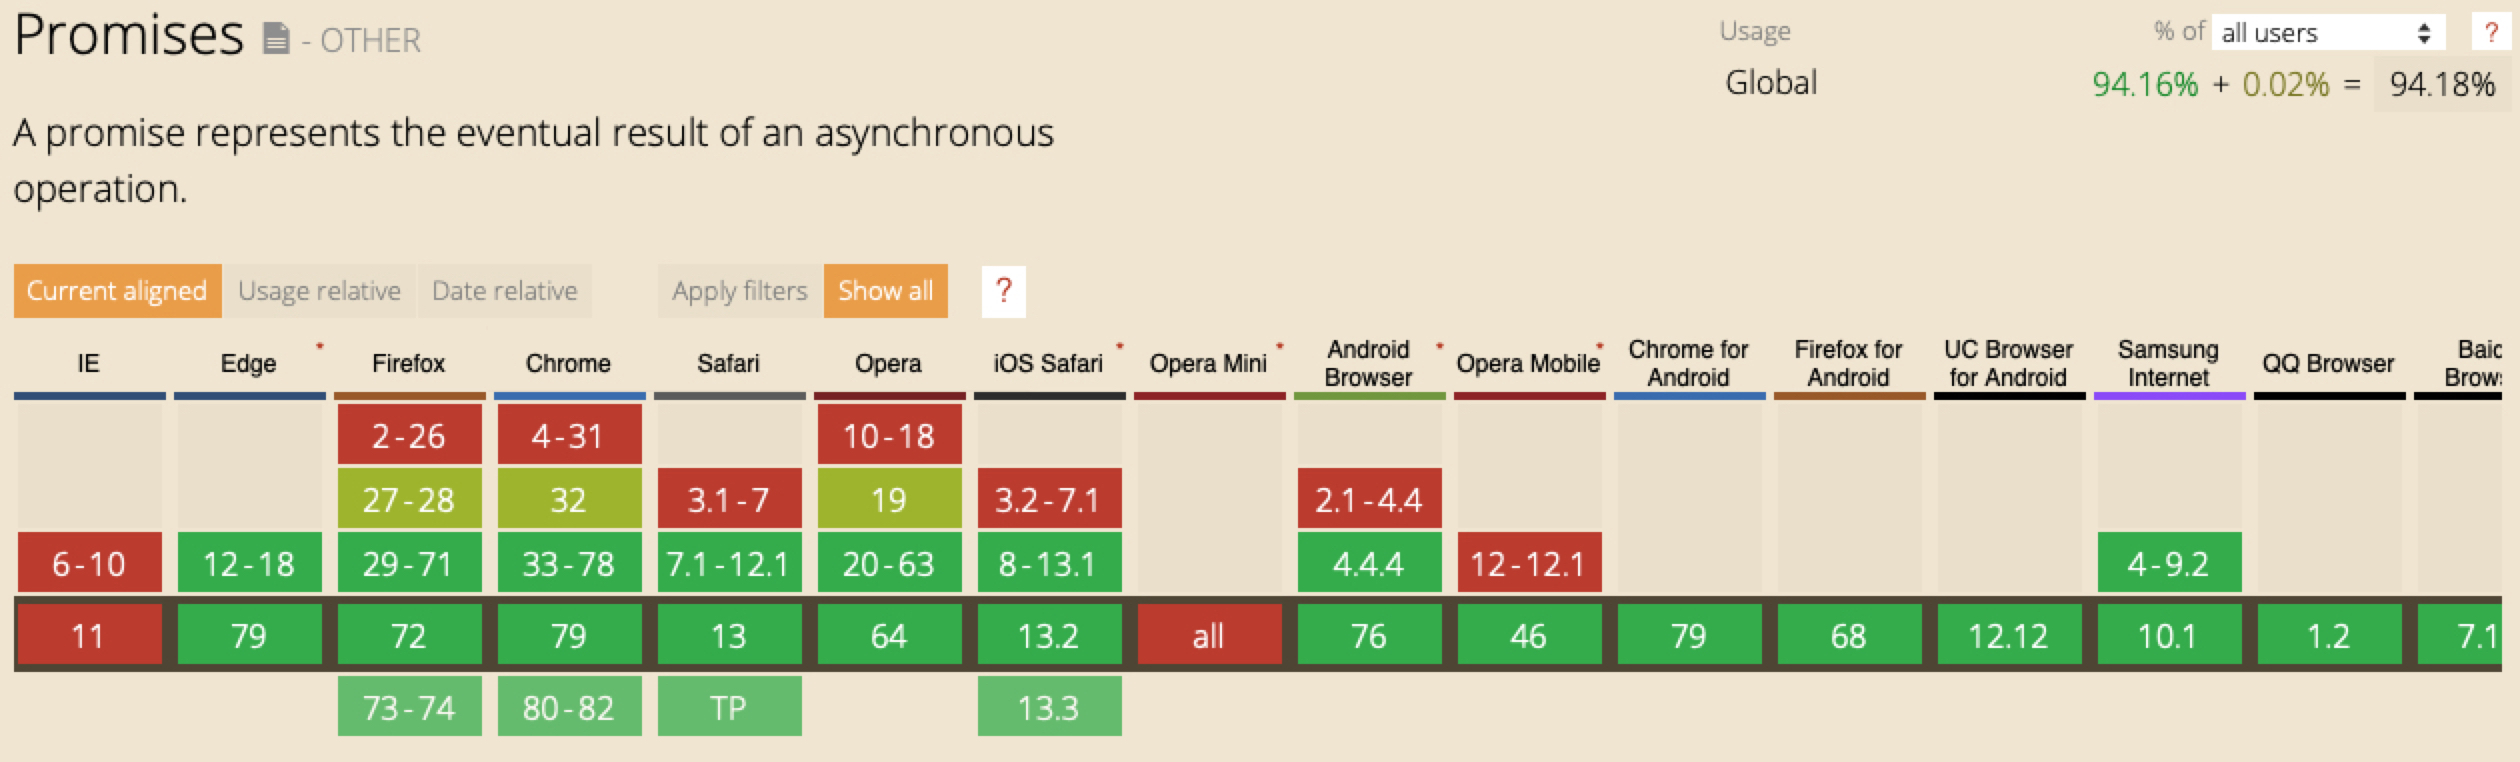
\includegraphics[width=0.8\linewidth]{assets/caniuse-promises.png}
  \caption{Browser support for JavaScript Promises}
  \source{https://caniuse.com/\#feat=promises}
  \label{fig:caniuse-promises}
\end{figure}

Developers often build a software project on top of a library or framework that handles all the infrastructure setup and allows the developers to focus on the main business logic. The POS application, for example, uses the Java Spring Framework. For the client-side of web apps, there are currently three big frameworks, namely React, Vue, and Angular, with React being the most popular, according to The State of Javascript Survey 2019, see figure \ref{fig:frontend-framework-usage} ~\cite{stateofjs.2019}. At first, I wanted to use Angular because the current Docify team who are also developing their application on a three-layer architecture with JavaScript for both client and server are using Angular as their client-side framework. However, after spending some time working with the framework, I decided to switch to Vue since Angular has a pretty steep learning curve, and I had already advanced experience with Vue from previous projects. Because the time for this thesis is limited to four months and the result is supposed to be a proof of concept, I felt justified in using a technology that I am more familiar with even though the local developer team at Capgemini is using a different framework.

\begin{figure}[ht]
  \centering
  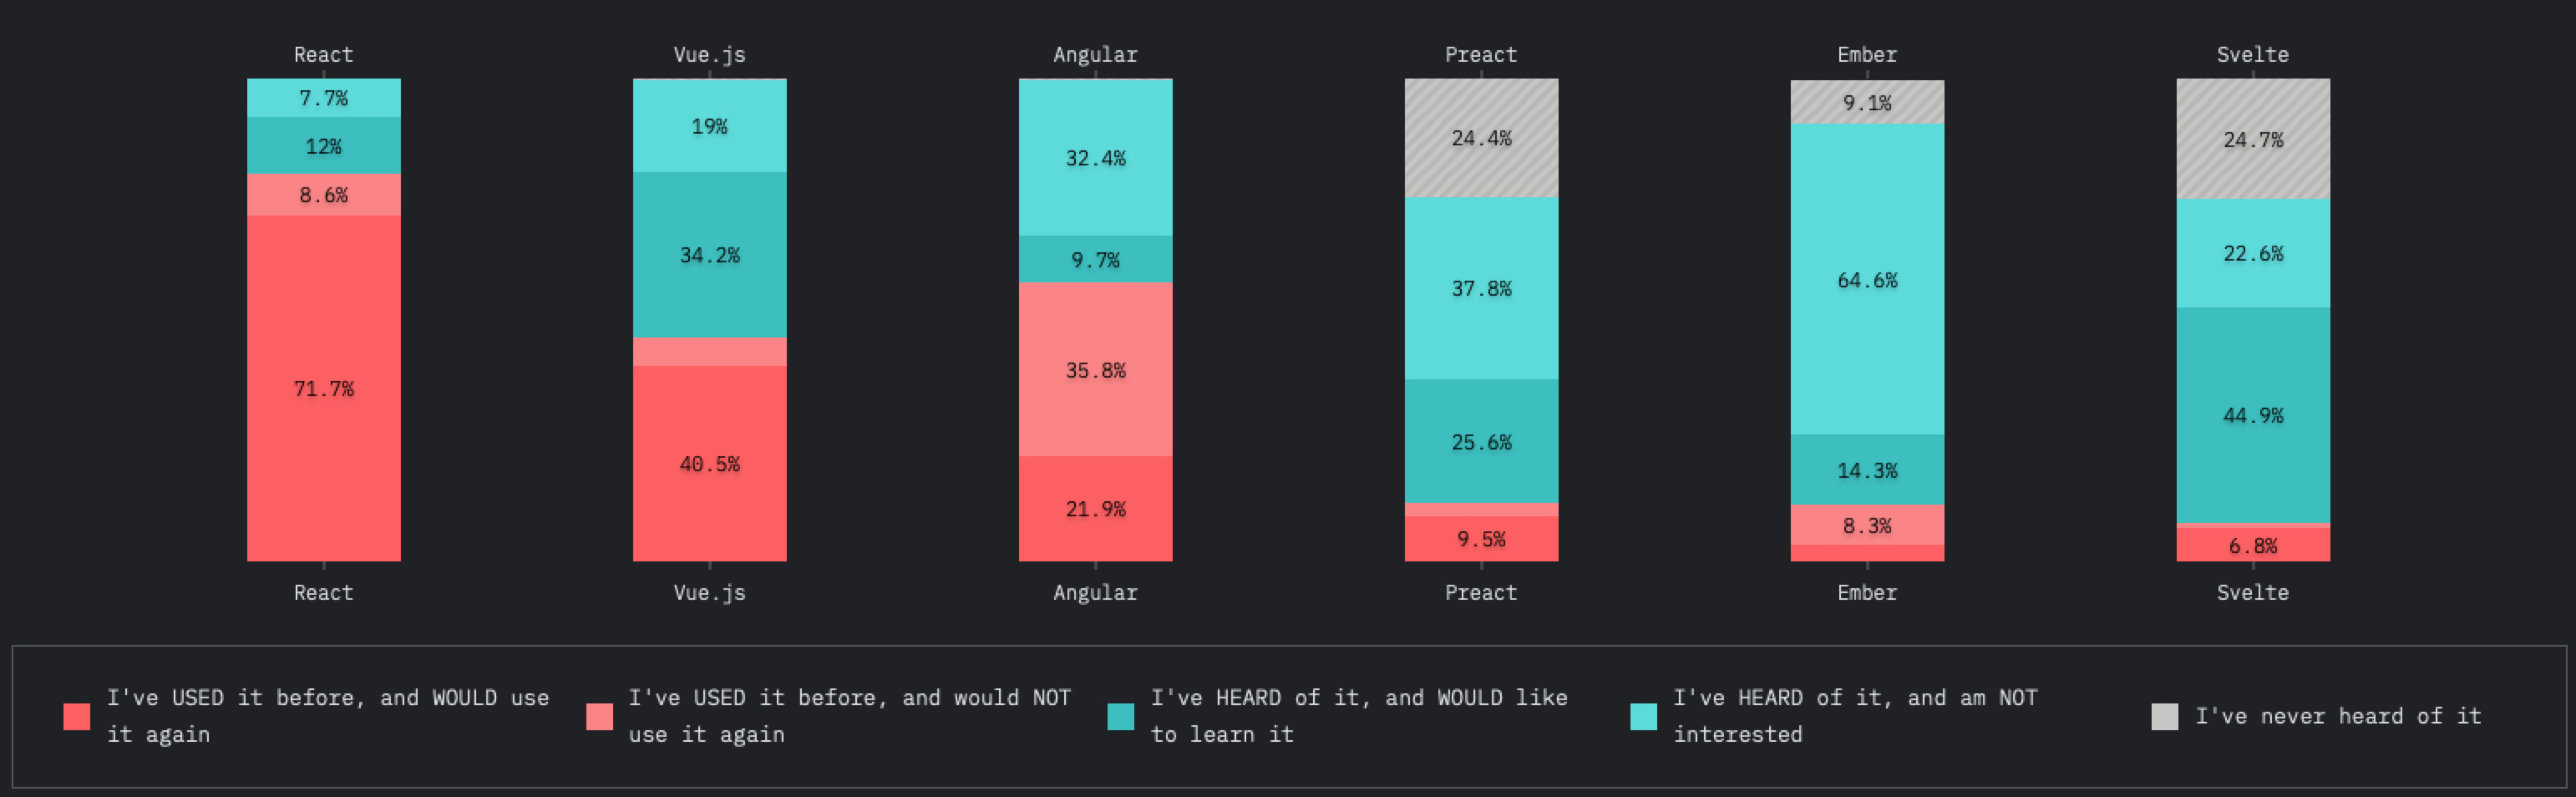
\includegraphics[width=0.8\linewidth]{assets/frontend-framework-usage.png}
  \caption{Usage statistics of current front end frameworks}
  \source{https://2019.stateofjs.com/front-end-frameworks/}
  \label{fig:frontend-framework-usage}
\end{figure}

Node.js is a runtime allowing the use of JavaScript on the server-side. Because the client-side of a web app has to use JavaScript, it is also an excellent choice for the server-side, thus the team only needs to have expertise in one programming language. The server-side framework the Docify team is using is called Express and is with 96\% awareness among JavaScript developers, basically the bread and butter tool for such a task ~\cite{stateofjs.2019}. The reason I am always referring to the Docify team is that, as already mentioned, they are the other microservice team using a JavaScript technology stack on the POS project. They are, therefore, my reference and, most likely, the people that continue the development of CEMicro after I finished.

PostgreSQL is the database that I am going to use for the data layer of CEMicro. It is the up and coming open-source relational database with a robust set of features ~\cite{stackoverflow.2019}. There are other databases out there like the more common MySQL and MongoDB, that uses an object-based system geared towards development with JavaScript. However, since once again, the Docify team is running PostgreSQL and the CEMicro service had no extraordinary requirements towards data persistence, I felt not much need to choose any other database system.

I want to mention one more technology outside the three-layer structure, which is vital to the idea of my task, and that is virtualization or containerization software. In the theoretical section about which problems microservices solve on page \pageref{sec:theory:what-problem}, one strong point in favor of this architecture model is the scalability argument. But for a service to be scalable, especially automatically in reaction to load, there needs to be a way to start and stop an instance of that service without manual interaction. Containerisation is not the first concept making this possible but by far the most sophisticated one. A container is an instance of a service that is self-contained, meaning it contains all the parts the software needs to run independently of the setup of the server. With the right software, such a container can then be started on any device and copied as often as needed. The right software for this is Docker, which has become the de-facto standard for containerization and is the most loved platform for this purpose among developers ~\cite{stackoverflow.2019}.

From the get-go, I developed CEMicro in a way that it can later run inside Docker containers. That means if you want to run CEMicro in the future, instead of needing to understand each technology and how to run it on your machine, all you needed is one docker command, and the app is ready for use.


\section{Designing the User Interface}

\begin{itemize}
  \item \done{How can the complexity of CEs be exposed more straightforwardly?}
\end{itemize}

The user interface doesn't just serve an aesthetic purpose; it helps the user to understand and manage the complexity of a system. Figure \ref{fig:pos} on page \pageref{fig:pos} and figure \ref{fig:ce-properties} on page \pageref{fig:ce-properties} show glimpses of the existing user interface in POS. The existing interface is functional but clunky and hard to use. For example, it is not immediately apparent that the validity date of a CE can be changed and how to do it. It is also difficult to understand which of the CE items is active under which circumstances.

Figure \ref{fig:mockup} shows a high fidelity mockup I created before even starting to implement the microservice. I showed it to my mentor and the Docify team to get their feedback on the design. I tried to make the relationship between CEs and templates as simple as possible. Each CE can contain individual items, so I tried to show their hierarchy clearly. I also wanted to make all the different properties as evident as possible, showing them in a condensed view, highlighting the ones that differ from default values and only showing input options when the item is in edit mode.

\begin{figure}
  \centering
  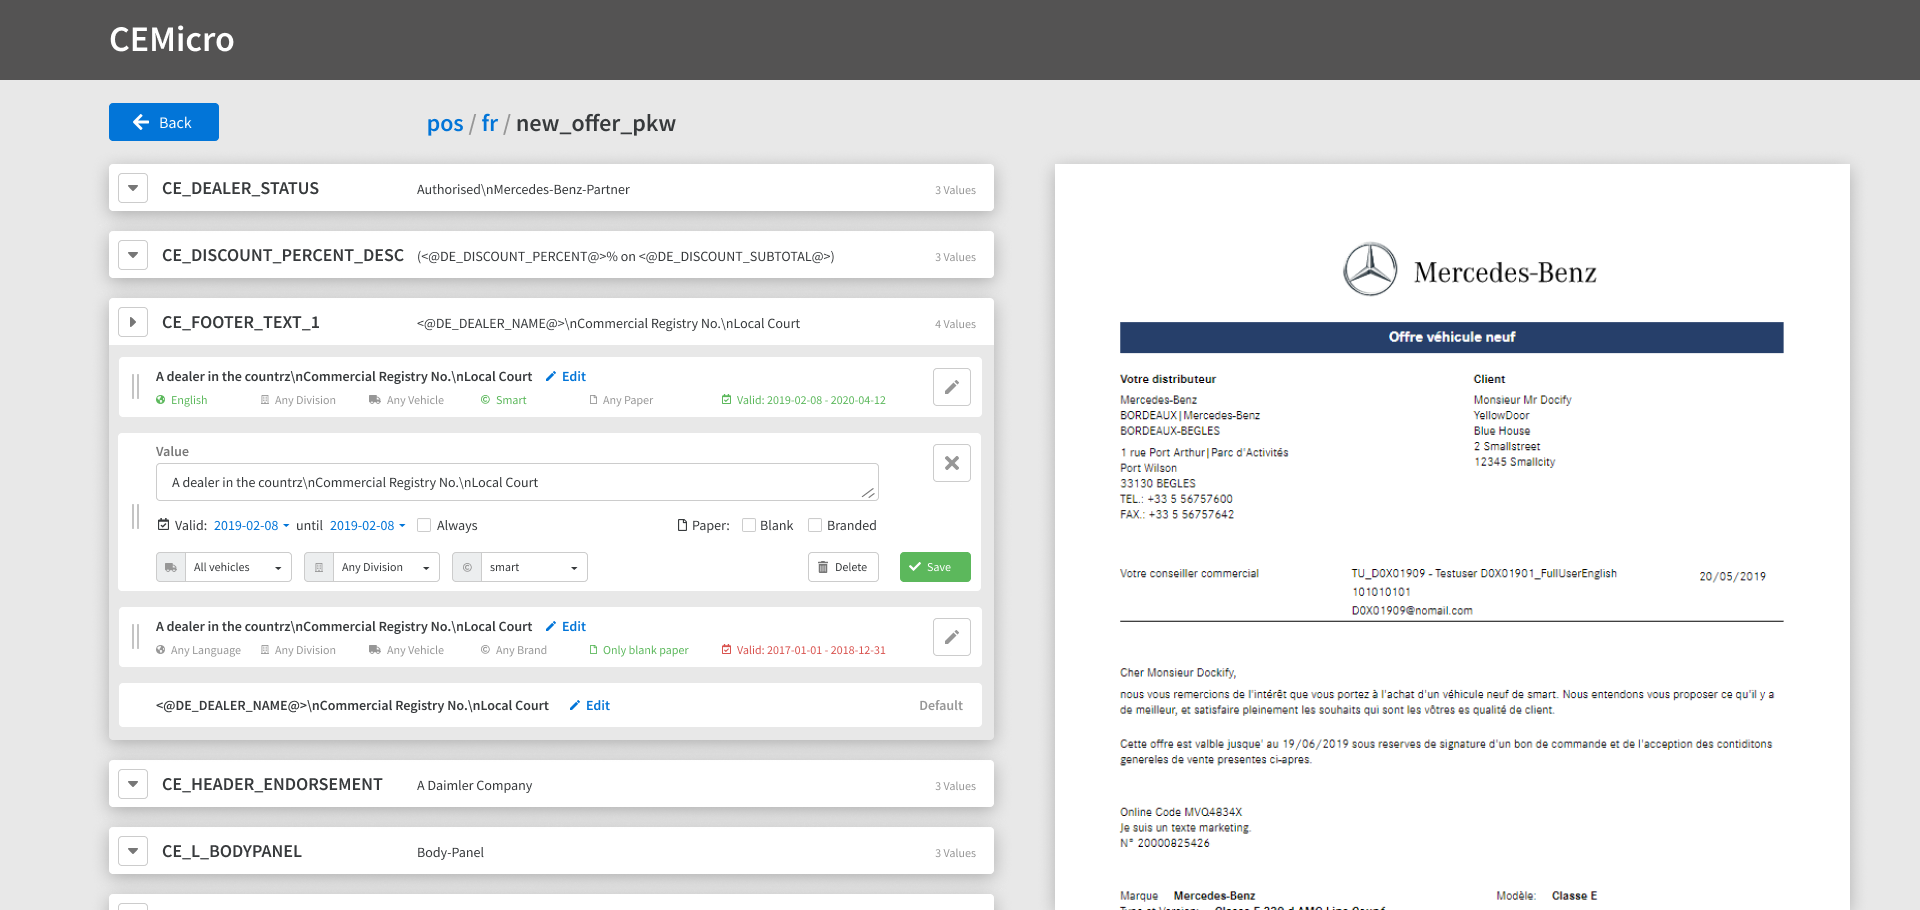
\includegraphics[width=\linewidth]{assets/cemicro-ui-mockup.png}
  \caption{User Interface mockup for CEMicro}
  \label{fig:mockup}
\end{figure}

In the final implementation, I decided to go with three views, always clearly showing the current position with breadcrumbs on top:

\begin{itemize}
  \item A list of templates (see figure \label{fig:cemicro-template-list})
  \item A list of elements per template (see figure \label{fig:cemicro-element-list})
  \item A list of items per element (see figure \label{fig:cemicro-item-list})
\end{itemize}

The controls of a single element item became a little more uniform in the end. I also added a ``Refresh'' button above the document preview to see the current changes applied. I am planning another set of controls next to the refresh button to choose the properties (new vehicle vs. used vehicle, etc.), which should be applied to the preview to see which item is used under which circumstances. This last feature, however, is not yet implemented at the time of this writing.


\section{Wrap-up}

This part of the project, investigating the existing application, and making architectural decisions, provided the most learnings for me. The theory behind microservices was comparatively easy to understand because I worked a lot with cloud infrastructures before. The implementation was simple because I have ample experience in programming at this point. It was interesting how much complexity accrued over time in such a simple feature as the configurable elements. Deciding where the data should live helped me better understand how distributed data works. And redesigning an existing user interface is something I like doing.



\chapter{CEMicro Implementation}
\label{sec:impl}

In this chapter, we dive into the practical implementation of CEMicro. The microservice consists of three layers, the frontend, the backend, and the database. Each layer is treated in some detail. Though the information is very technical, I made an effort to keep it simple enough for less technical affine readers to understand. In no way does this chapter cover the implementation comprehensively but provides an overview of the most critical decisions.


\section{Setting up the Development Environment}

It seems trivial to treat the development environment in this chapter, but that would be a disservice to any programmer. The development environment is an essential part of writing an application and can be as much of a time sink as software bugs, as we will see. I am used to developing on a Mac operating system. Mac is based on Unix and offers a built-in Bash shell, basically just like any Linux machine, while Windows uses an entirely different foundation for its operating system. All the technologies which work with cloud computing and distributed services operate on Linux systems because the internet runs on Linux\footnote{Yeah, sorry Microsoft}. We are talking about technologies like Git version control, Docker container virtualization, and Node.js and its packet manager NPM. The machine Capgemini provided me with is a Windows computer.

I first set up Visual Studio Code, currently the most popular code editor, especially among web developers and developed by Microsoft ~\cite{stackoverflow.2019}. Next, I set up git\footnote{https://git-scm.com/downloads}, which comes with a complete Bash environment, howbeit with a reduced feature set. Bash stands for ``Bourne Again Shell'' and is a variation of the default Unix shell, a command-line interface. An average user usually never uses the command line but interacts with generated user interfaces (GUI) of a program. In a shell, the user can interact with programs by typing one-line commands. For example, \inlinecode{rm -rf test-dir/} instructs the simple ``remove'' program to delete the ``test-dir'' folder with all its content. This way of using programs is handy for programmers and system administrators in their work, especially if running commands on remote computers through SSH\footnote{Secure Shell, a way to use the shell of a remote computer} sessions.

\begin{figure}[ht]
  \centering
  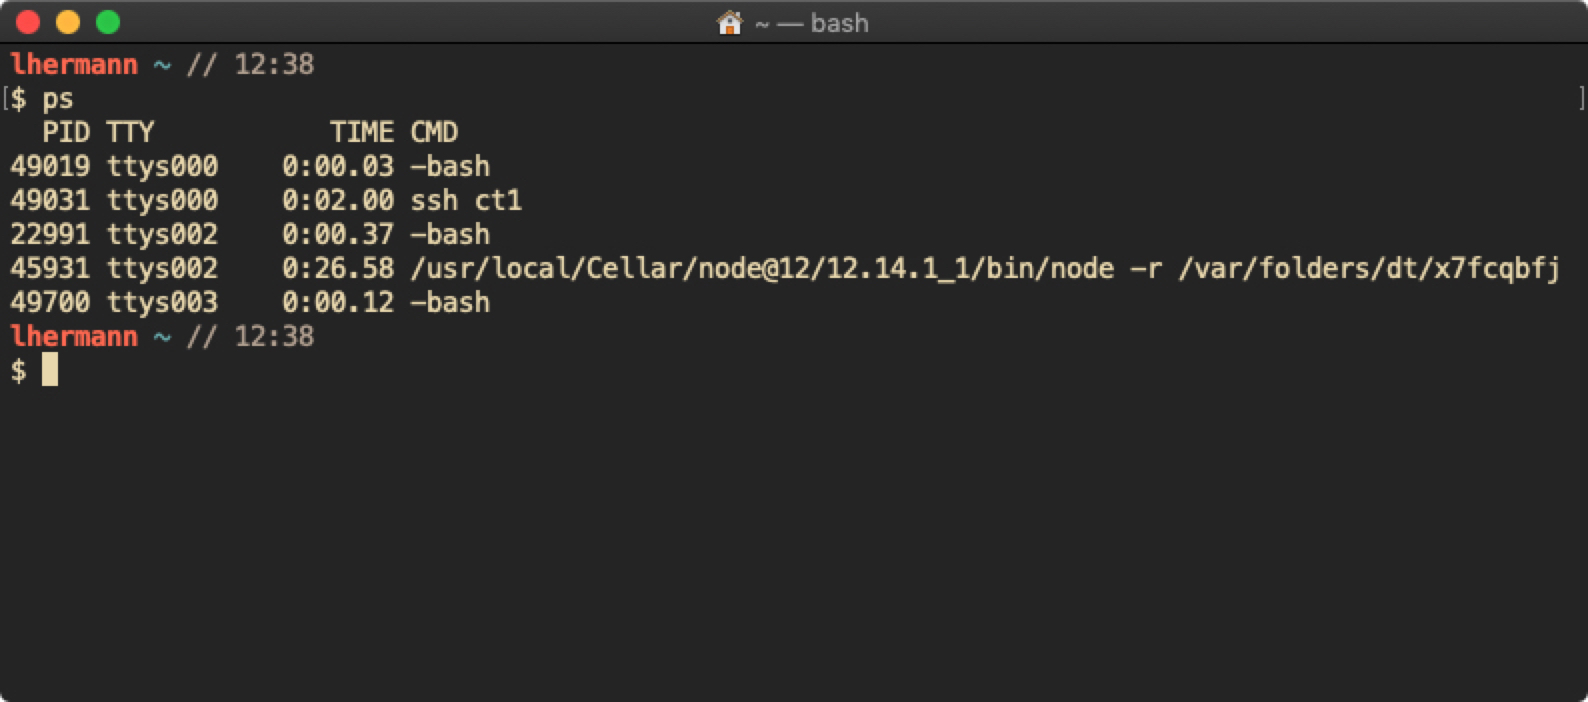
\includegraphics[width=0.75\linewidth]{assets/example-bash-window.jpg}
  \caption{Example for a bash terminal executing the 'ps' command}
\end{figure}

Because I planned to write the entire application in JavaScript, I set up a Node.js environment\footnote{https://nodejs.org/}. JavaScript is an interpreted language; it means that the code does not need to compile to machine code like Java, for example, but the Node runtime reads the JavaScript file and translates it for the computer on the fly. It means that I can start a program by simply typing \inlinecode{node main.js} into the shell, which then executes the contents of main.js. Furthermore, I can install a JavaScript tool like Nodemon\footnote{https://www.npmjs.com/package/nodemon} with \inlinecode{npm install nodemon} that watches the JS\footnote{JS is short for JavaScript} files on my systems and restarts the application whenever I change the file. This provides instant feedback, in the form of an updated application or error messages, and makes development comfortable.

\begin{figure}[ht]
  \centering
  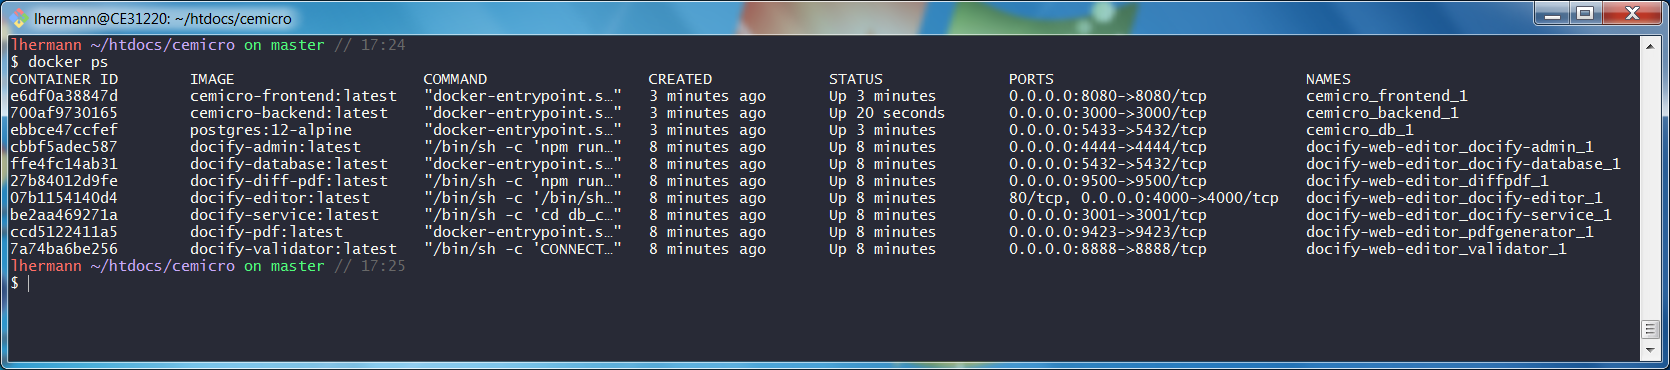
\includegraphics[width=1\linewidth]{assets/terminal-docker-ps.png}
  \caption{'docker ps' shows all running docker containers}
\end{figure}

Docker\footnote{https://www.docker.com} is a tool that can run the software in a container. A container is like an application that brings its entire ecosystem with it, howbeit a very simplified one, so that it doesn't become too large. This application then runs in isolation from anything else on the host system. This is very useful because it allows the developer to run dependencies like databases or other services for an application without the hassle of installing them on the system manually and the difficulty of handling different versions. For the development of CEMicro, I ran my PostgreSQL database in a docker container. I also needed a running instance of the Docify service, itself a combination of six containers, which I downloaded and started in Docker. The \inlinecode{docker-compose} command provides a very convenient way to start all required containers for an entire application at once. These containers then run in the background, and the developer can concentrate on his current code.

One challenge I faced with setting up bash on windows was the limited way in which the shell environment of the git application works. Familiar commands and shell setups on Unix machines were not available under the Windows environment, and it took me a while to work around this limitation. Another problem arose with Docker in that it works with Unix file system permissions. On a Unix system, every file has a set of nine permissions, read, write and execute separate for the user, the group and others\footnote{The details about Unix file permissions go beyond this chapter, for more info see https://www.tutorialspoint.com/unix/unix-file-permission.htm}, this system is part of the hard drive format and OS kernel\footnote{A kernel is the bottom-most layer of an operating system}. Windows does not have any file system permissions; it's not part of the operating system. Instead, Windows handles users and groups with dedicated services, and this is also the reason why there are so many more worms and viruses for Windows. The Docker environment for Windows fakes those permissions. But for specific requirements, for example, when using Docker volumes, these permissions need to be changed to work. It is possible to do this, but I couldn't find out how and I assume it has to do with a user management service, which is not accessible under the closed business setup of the machine Capgemini gave me. It, therefore, took me a while to find a workaround for Docker volumes so that they only exist within the virtual environment and don't come in contact with the Windows host.

\section{Application Programming Interface}
\label{sec:impl:api}

The CEMicro service deals with three different objects\footnote{In programming, an object is like a container for data.} — the template, the configurable element, and its items. The template contains the template string in combination with sample data for the placeholders inside the template. The configurable element, as discussed in the section on page \pageref{sec:arch:understanding}, a holder for the individual properties as well as the name and the default value. And the configurable element item which is one individual set of the properties of table \ref{table:ce-properties}.

\begin{table}[!ht]
  \begin{center}
    \begin{tabular}{|l|l|p{6cm}|}
      \hline
      Action & Route & Description \\
      \hline\hline
      GET & /templates & Get a list of template abstracts \\
      \hline
      GET & /templates/\{market\} & Get a list of template abstracts by market \\
      \hline
      GET & /templates/\{market\}/\{name\} & Get a template by market and name \\
      \hline
      GET & /templates/\{market\}/\{name\}/pdf & Get the PDF of a template by market and name \\
      \hline
      GET & /configurable-elements & Get a list of Elements for the given parameters \\
      \hline
      GET & /configurable-elements/\{id\} & Get an Elements by id \\
      \hline
      PATCH & /configurable-elements/\{id\} & Update an Element by id \\
      \hline
      GET & /configurable-elements/\{id\}/items & Get all Items for an Element \\
      \hline
      POST & /configurable-elements/\{id\}/items & Create an Item for an Element \\
      \hline
      GET & /configurable-element-items/\{id\} & Get an ElementItem by id \\
      \hline
      PUT & /configurable-element-items/\{id\} & Update an ElementItem by id \\
      \hline
      PATCH & /configurable-element-items/\{id\} & Patch an ElementItem by id \\
      \hline
      DELETE & /configurable-element-items/\{id\} & Delete an ElementItem by id \\
      \hline
    \end{tabular}
  \end{center}
  \caption{API endpoints of the CEMicro backend}
  \label{table:api-endpoints}
\end{table}

Table \ref{table:api-endpoints} shows all the API endpoints of CEMicro. We can see that a market-name tuple uniquely identifies a template. That means a template name itself is not unique because two markets, like the Netherlands and France, can use the same template name. To make sure these templates do not get mixed up, they are namespaced by the market. Also, observe that there is no POST or PUT actions for templates, that's because templates are not saved in the CEMicro database but fetched from the Docify service whenever requesting this endpoint.

One important concept is the single source of truth, meaning that one piece of information only exists in one place. This is especially important when working with microservices and other concepts of distributed architectures. Since the services and thus the programming logic is distributed, information, by necessity, also needs to be distributed. However, as just established, we do not want duplication of information. Thus, with microservice architectures, one piece of information should only exist inside a single microservice. CEMicro solves this the single source of truth principle by requesting templates on the fly from the Docify service and only saving configurable elements and their items in its database.

Initially, I planned to include templates in the database because it is such an essential part of the application. The frontend needs to list all the available templates, and configurable elements are essentially placeholders within the template. However, saving the templates in our database would mean duplication of the information because Docify handles them. It would be possible for docify to send a notification to CEMicro whenever a template changes, but the easier way is to fetch templates fresh every time we need them.

Both elements and element items are saved in the CEMicro database and entirely managed by it. It is common to provide CRUD actions for every resource. CRUD stands for CREATE-READ-UPDATE-DELETE, the four principal actions for data. In the table, we can see that element items have all four CRUD operations plus PATCH, which is a partial update function where only a subset of properties has to be provided. Configurable elements, however, do not have four CRUD operations. That's because I decided to create them on the fly. Whenever the user opens a template in the frontend, it requests all the elements from the backend. At that point, the backend parses the template string for a list of all the necessary configurable elements. It then compares this list with the database and creates an element that is missing before returning the complete list of elements to the frontend. This way, the user is saved the hassle of manually creating an element after adding it to the template in Docify. It saved one working step. However, during the debriefing with the project manager, we concluded that it would be better to additionally offer the manual option to the user so he can create and delete elements as needed.

\begin{figure}[ht]
  \centering
  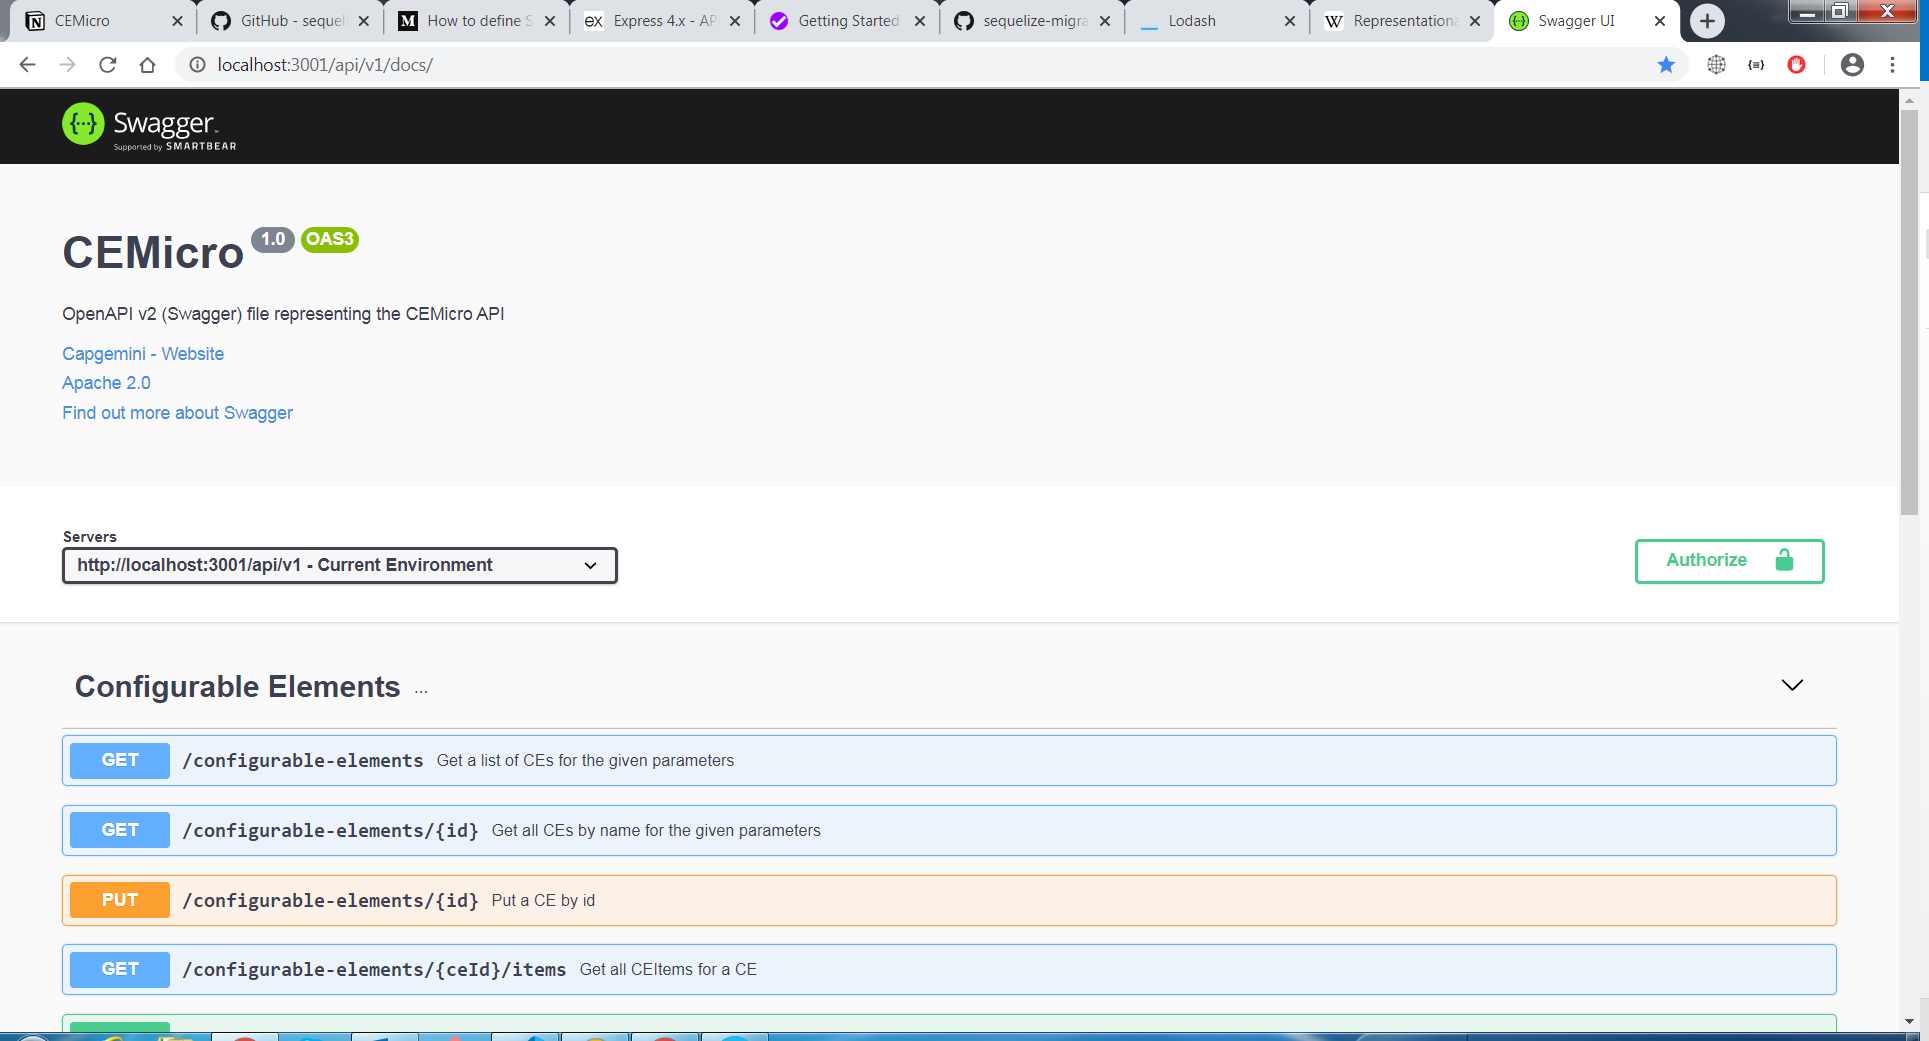
\includegraphics[width=0.8\linewidth]{assets/swagger-api-docs.png}
  \caption{Interactive API documentation with Swagger}
  \label{fig:api-docs}
\end{figure}

The appendix \ref{sec:appendix:openapi} shows an excerpt of the \inlinecode{openapi.yml} file. This file is the authoritative documentation for the API. Swagger\footnote{https://swagger.io}, the open-source project behind the OpenAPI standard, provides tools to generate an interactive documentation page from this file automatically, see figure \ref{fig:api-docs}. Docify uses a library called ``swagger-tools'' to automatically generate some scaffolding for their code directly from their OpenAPI file. This approach saves some repetitive coding and helps to tie the functional code and the documentation together. For CEMicro, however, I decided to omit this library and add everything by hand because the project is stale, it didn't see any updates for two years, and does not support the latest version of the OpenAPI specification\footnote{See https://www.npmjs.com/package/swagger-tools}.


\section{Backend Framework with Express.js}

I tried to mostly include libraries that the Docify team already used to make the transition more manageable, and so that the two microservices can merge with little friction if desired. Fortunately, Docify tended to use the bread and butter libraries for JavaScript servers: Express ~\cite{stateofjs.2019}. Express\footnote{https://expressjs.com} is a minimalist Node.js framework that takes care of HTTP requests and routing with no additional frills. Besides, Express leaves a free choice of the file structure.

\begin{figure}[ht]
  \centering
  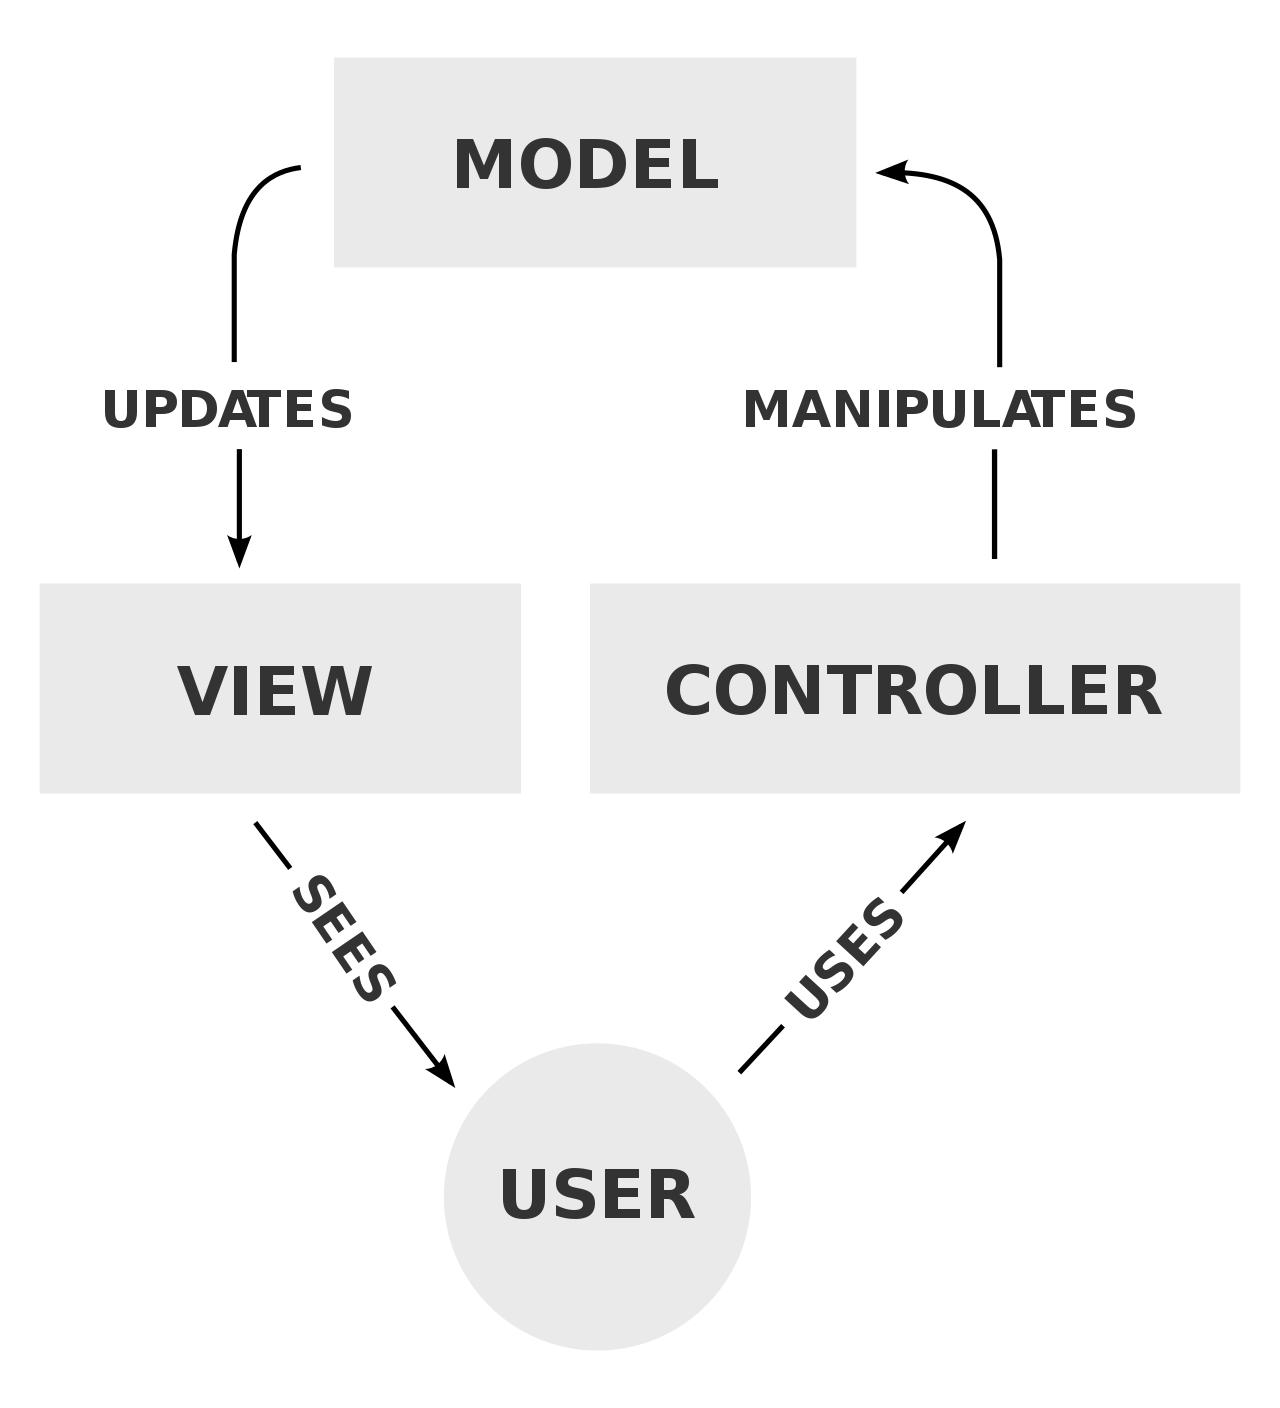
\includegraphics[width=0.3\linewidth]{assets/mvc-process.png}
  \caption[Diagram of interactions within the MVC pattern]{Diagram of interactions within the MVC pattern ~\cite{mvc.wiki}}
  \label{fig:mvc-process}
\end{figure}

In backend development, it has become common to use the Model-View-Controller (MVC) architecture. User interactions go to the controller, a function that decides which data models to load and what view to show to the user. A view is a general word for a page of an application. In pure API backends, that is, backends that don't render a view but only provide an API, the view layer is usually omitted. The controller directly returns the data to the caller of the API.

Additionally, a service layer is often used between the controller and the model. The controller calls the service to get the data it needs. The service is responsible for the core business logic, loading the data from the database by calling the model, and then performing the necessary data manipulations. Appendix \ref{sec:appendix:mvcs} shows a code example for the controller, service, and model of the element component. Sequelize\footnote{https://sequelize.org/v5/}, an ORM\footnote{Object-relational mapping, see https://en.wikipedia.org/wiki/Object-relational_mapping} library for Node.js, handles the data model and database access; see the next section.

There are three additional preliminary concerns for every server-side application. The first is data validation for which I used the express-validator\footnote{https://express-validator.github.io/docs/} library. It takes care that the parameters provided by the user can be processed and don't contain any malicious code. The second concern is user access management, which we decided to omit because of the brevity of the provided time. We also decided to omit the third concern, which is testing. Omitting tests is considered a developer sin, but because CEMicro is more a proof of concept, we felt comfortable in saving the development time.

\section{Data persistance with PosgreSQL}

All the decisions for which data goes where were made at this point, which makes the database implementation trivial. As mentioned in Section \ref{sec:arch:technology} I decided on PostgreSQL. Setting up the database itself at this point means starting a Docker container with the official PostgreSQL Docker image\footnote{https://hub.docker.com/_/postgres/}. The challenge with databases lies in keeping the schemata up to date with the data model of the backend. For programming code, git version control keeps track of all changes and can handles conflicts when two developers edit the same lines of a file simultaneously. With git, every programmer can always pull the current version of the code from a central repository. Such a system doesn't exist for databases. Instead, developers write migrations, a set of instructions to bring the database schema from an older to a newer state. These migrations are committed to version control so that developers can update their local database as needed. I looked at several migration solutions for Node.js.

The Docify team recommended Flyway\footnote{https://flywaydb.org} to me, but it is primarily for Java applications, and I couldn't find a suitable package for Node.js. Another recommendation I found was Umzug\footnote{https://www.npmjs.com/package/umzug}, a well-supported package, but it doesn't handle the actual database manipulation. The documentation for Umzug recommended the Sequelize ORM\footnote{https://sequelize.org/v5/} to interface with the database. After looking at Sequilize, I realized that it provides a database-agnostic ORM, which means that I can write database access in its custom format, and Sequilizes translates it into valid SQL statements for PostgreSQL. Not only that, Sequelize makes it trivial to change the database dialect, for example, from PostgreSQL to MySQL, with a simple configuration option, and it takes care of the rest. And Sequelize comes with its system for database migrations, which I decided to use.


\section{Frontend Framework with Vue.js}

Originally the plan was to write the frontend in Angular\footnote{https://angular.io}. Angular is a client-side framework created by Google and popular among more traditional software companies for its Java-like approach in the directory structure and use of the static type JavaScript language extension Typescript. I agreed with this decision, primarily because the Docify team also used it. I am mentioning the Docify team repeatedly here for the mere reason that it is the only other service inside the POS team written with modern web-development principles. It is the only other microservice inside POS in existence. However, Angular turned out to have a rather steep learning curve and is overly complicated for such a small application as CEMicro. After completing several tutorials, I understood why 35\% of frontend engineers say they used Angular and would never use it again\footnote{See figure \ref{fig:frontend-framework-usage}}. Having said that, I realized I already mentioned this in the previous chapter, but it bears repeating.

Going with vue turned out to be a breeze. I already had ample experience with the framework and knew which plugins to include for the required use cases. Because CEMicro is a proof of concept, my mentor and I felt justified with the decision. I set up the frontend in such a way as to include the most commonly used techniques so that a rewrite into Angular by another team, later on, would be frictionless. For example, I exclusively used Bootstrap\footnote{https://getbootstrap.com} components for the user interface. Bootstrap is the go-to CSS framework for standard user interfaces like the admin page of CEMicro. Having a working user interface build on these principles as an example, the next team can rewrite it quickly if necessary.

I also made sure the frontend looks almost identical to Docify so it can be merged if desired and so that users already familiar with the Docify interface can use CEMicro intuitively.

\begin{figure}[ht]
  \begin{subfigure}[b]{0.5\linewidth}
    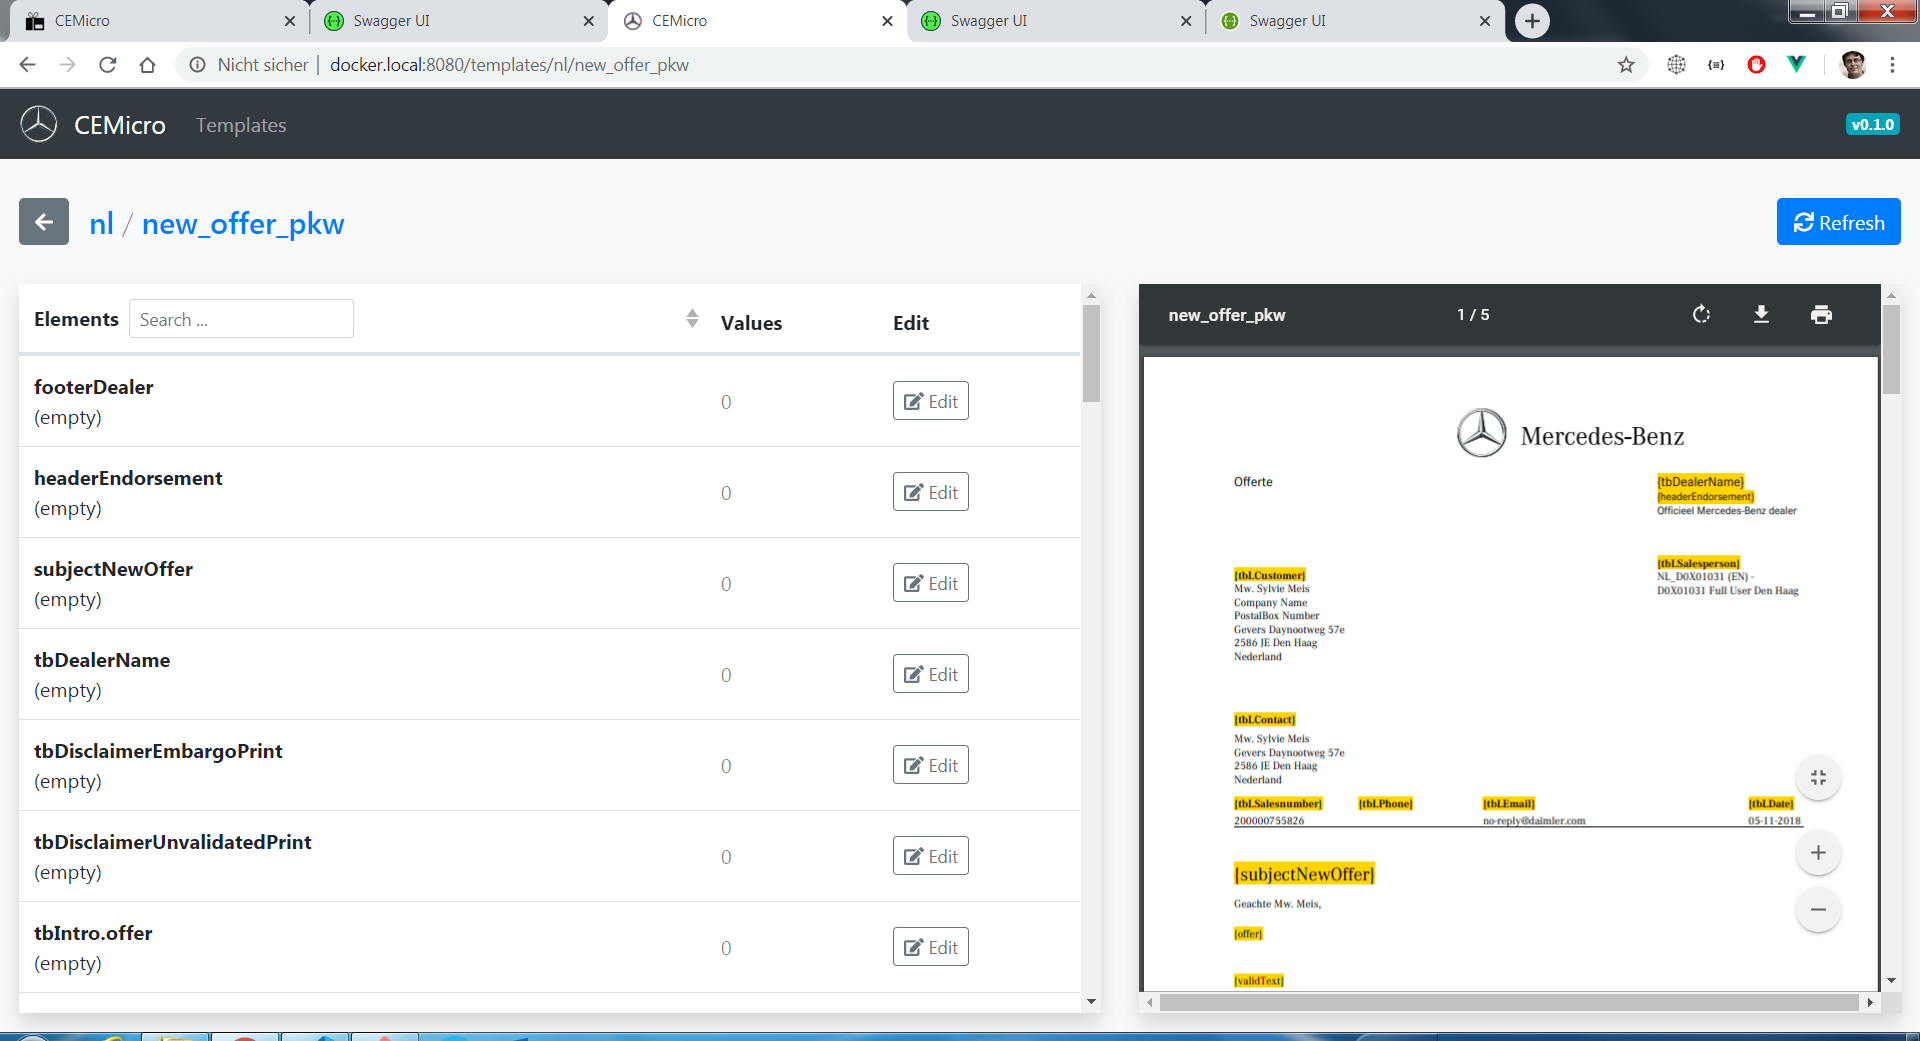
\includegraphics[width=\linewidth]{assets/cemicro-element-list.png}
    \caption{CEMicro element editor}
  \end{subfigure}
  \begin{subfigure}[b]{0.5\linewidth}
    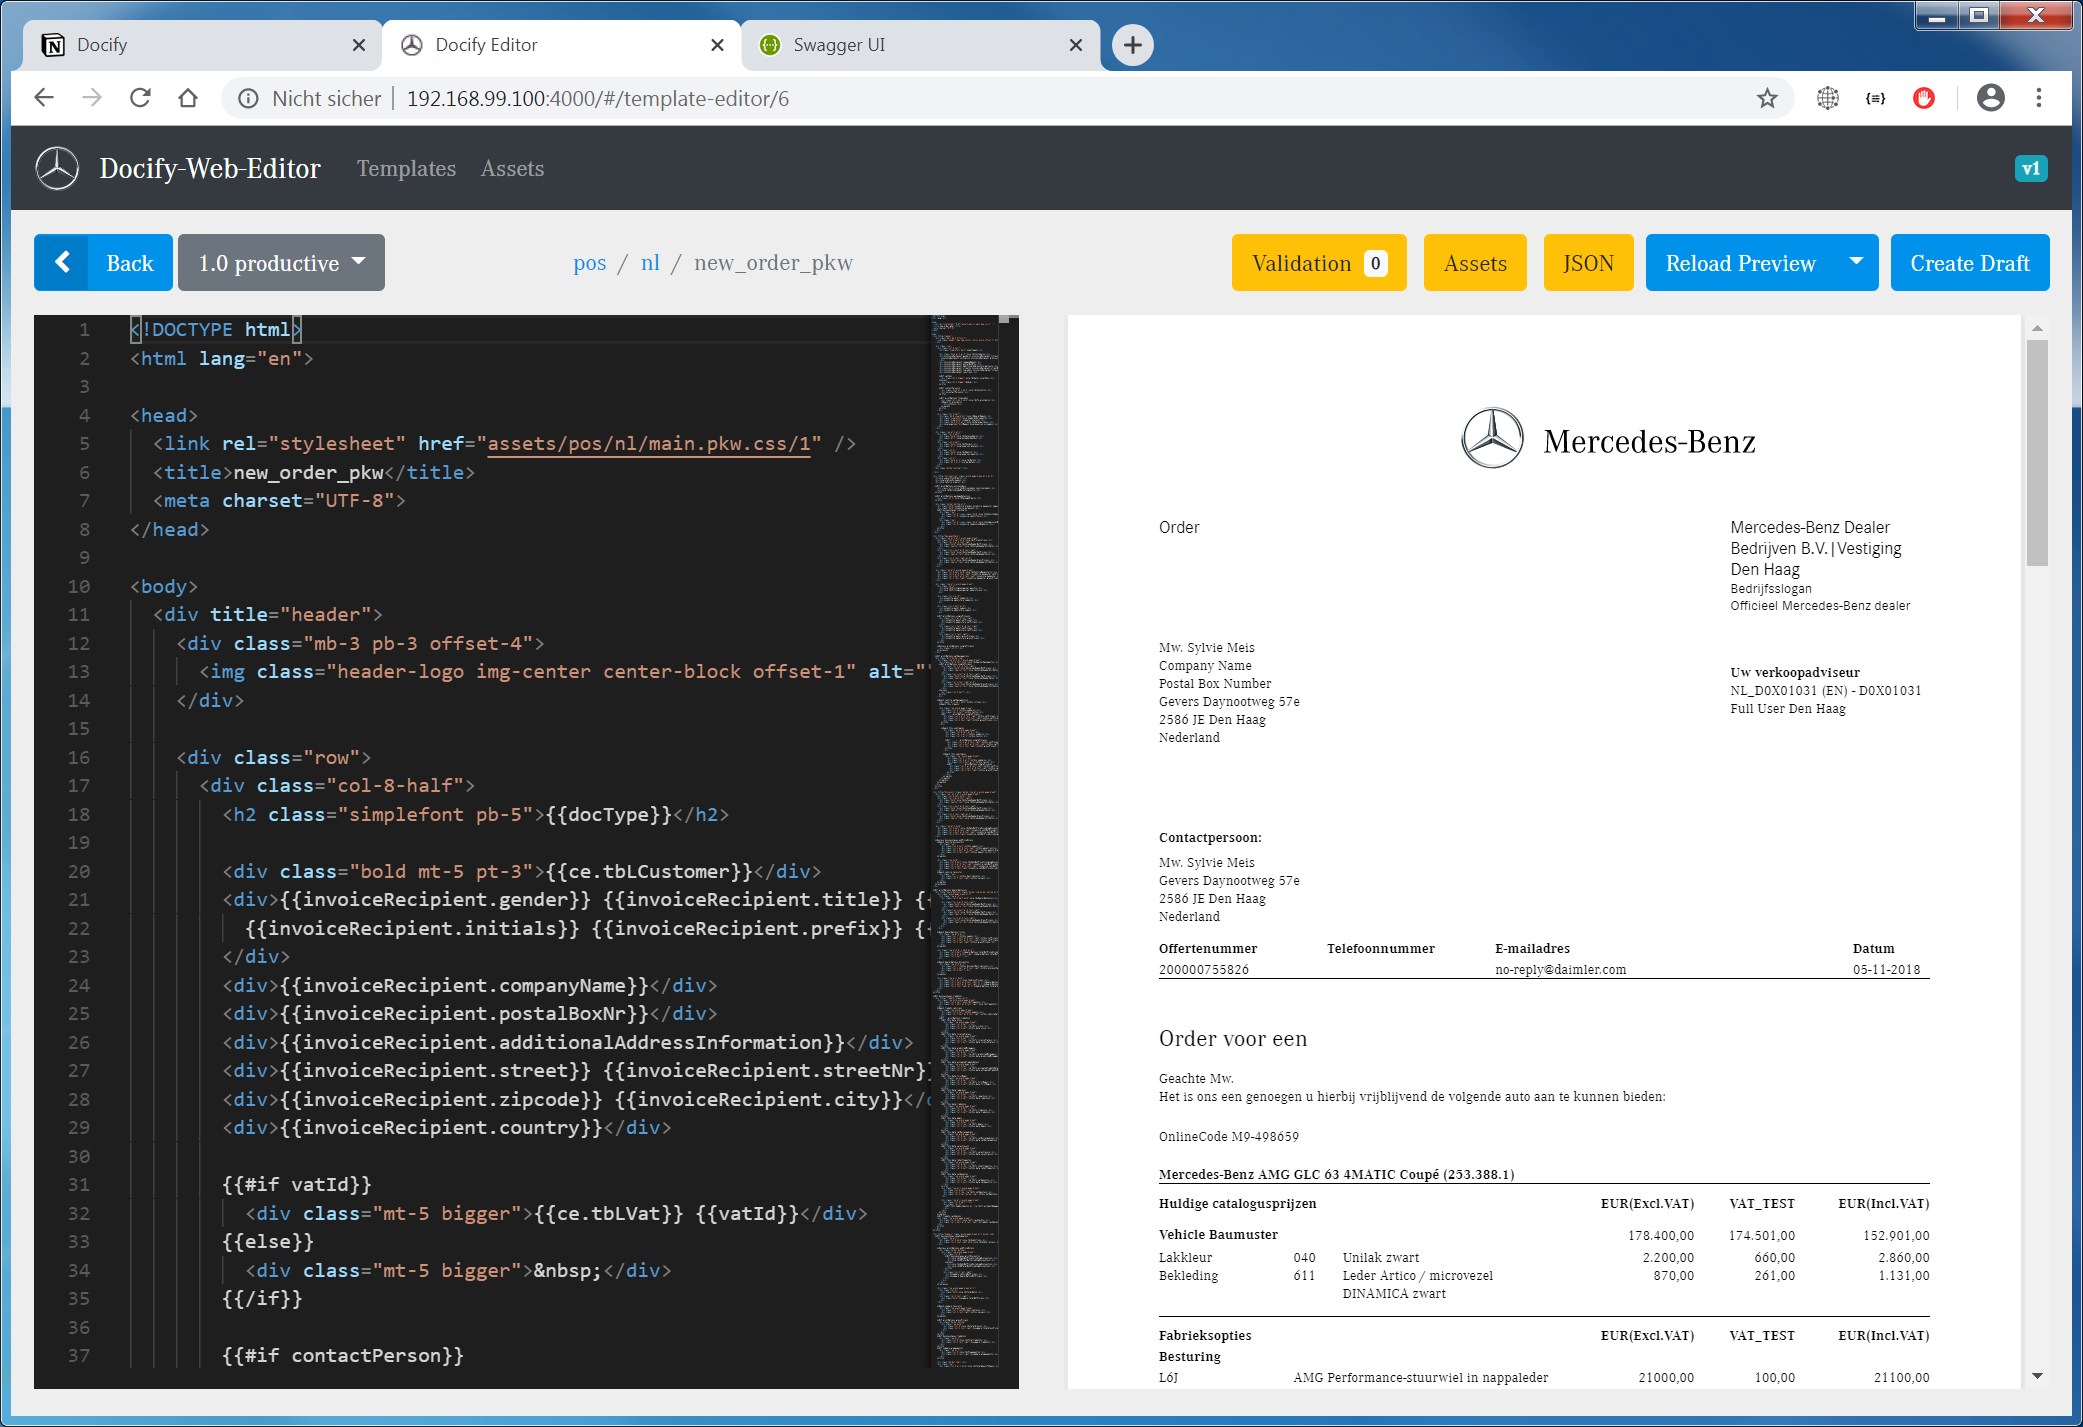
\includegraphics[width=\linewidth]{assets/docify-editor.png}
    \caption{Docify template editor}
  \end{subfigure}
  \caption{CEMicro's user interface is similar to that of Docify}
  \label{fig:cemicro-docify-ui}
\end{figure}


\section{Virtualisation with Docker}

If an application is packaged with Docker, then starting the application on a new machine is a breeze. PostgreSQL uses an official predefined Docker image, which works with minimal configuration, in this case, only a few environment variables. Both the backend and frontend use the official Node.js image. Only the image is not enough in this case because the programming code has to go into the container as well. One way to do that is with so-called volumes. A volume is a directory existing on the local machine and in the docker container at the same time. This arrangement is beneficial when using Docker during development but not for running it in production. I didn't use Docker during development because it tends to be a little slow. After all, the Docker volume has to sync the filesystem between the host and its virtual machine. Instead, I am running the application right on my system with my Node.js runtime, which is significantly faster. But for the production build, I want to have everything inside the container. To achieve this, we add a Dockerfile to the application, using the Node.js image as a foundation and building upon it with our code.

For example, here is the Dockerfile for the backend:

\begin{lstlisting}
FROM node:12-alpine

WORKDIR /var/app

COPY --chown=node:node . .

RUN npm install --production

ENV SERVICE_HOST=192.168.99.100
ENV SERVICE_PORT=3000
ENV NODE_ENV=production
ENV DB_HOST=db
ENV DB_USER=cemicro
ENV DB_PASS=123456
ENV DB_PORT=5432

EXPOSE 3000

USER node

CMD ./node_modules/.bin/sequelize db:migrate && npm run production
\end{lstlisting}

We can see that it uses the \inlinecode{node:12-alpine} image as a foundation, copies the files from the backend into the new image, and installs all NPM dependencies. It then defines some environment variables and instructs the container to run a set of commands when on start. An ``image'' in Docker language is like a blueprint, and a ``container'' takes that blueprint and creates a live instance from it. Multiple containers can be created from one image.

The backend is particularly simple because it doesn't require any build step; the code is just copied and executed directly. The frontend, however, posed an interesting challenge because a build step is required. The frontend is made up of special \inlinecode{.vue} component files which cannot be executed directly. First, we have to transform them into valid HTML, CSS, and JavaScript files during a build process. But to keep the image as small as possible, all the code that was only required for the build needs to be removed before finishing the Docker image. It turns out that NPm provides a command to ``prune'' development code from the filesystem after the build, here is the relevant excerpt of the frontend Dockerfile:

\begin{lstlisting}
RUN npm install
RUN npm run build
RUN npm prune --production
\end{lstlisting}

And with that, the containerization of the CEMicro application is complete. Now the single command \inlinecode{docker-compose up} takes care of building and starting all three parts of the application, including running the migrations for a new database, and it is then usable through the browser.


\section{Interfacing with the monolith development team}

Interfacing with the rest of the team was probably my most significant challenge in this task. Robin, my mentor, went to great length to make sure I had everything I needed and was taken care of. But even his endeavors can only go so far. In the end, I was part of my CEMicro team of one, only talking now and then with others from POS when necessary. This situation, of course, is particular to my position as a bachelor student with a project that only lasts four months, and yet, some lessons can be learned from it.

When extracting a microservice, as with any other software development, make sure there is a regular exchange of all the key parties involved. Don't only bring in the main stakeholder at the end of the project, as was the case with my project. Chances are once the boundaries are specified and understood, the team would want to simplify concepts that grew in complexity over the years. Take this chance, simplifying software is always a worthwhile endeavor.

Next, don't treat your microservice as not relevant. If your company wants to move forward, embrace change like this and take it seriously. I assume the problem was that Capgemini doesn't own the POS project itself but is doing client work for Mercedes Benz. It means the primary stakeholder is another layer removed from the actual developer. Instead of Mercedes wanting to invest in a service-oriented architecture, I had the impression that Capgemini tried to entice its client to do so. This situation was certainly not the most fertile ground for such technological innovation, especially since it doesn't translate into hard coin right away.

In the end, I did work with the team responsible for Docify. I tried to understand their application and their pain points. For example, Docify has two different user interfaces, one for administration and the other for daily use. Both users interfaced use their dedicated backend service. However, these two services use the same database. I asked about this arrangement, and they made it clear that this arrangement was the wrong choice and that these sub-services were cut too small. I also contributed to their codebase by adding a small API endpoint, which I needed for CEMicro. Beyond this, however, I worked alone.


\section{Documentation of CEMicro}

Documentation is a point not particular to microservices but probably of more importance here. Any application needs proper documentation, so new developers can hit the ground running. When using a microservice architecture, it is even more likely that programmers need to make changes that have never worked on the service before. This thesis is one way of documenting CEMicro and should work as a reference for others. More important, however, is to leave proper breadcrumbs where others would expect them.

Confluence is a kind of wiki page developed by Atlassian, the company behind Jira, which Capgemini uses for its project management. It is the place where the entry point for everything POS can be found, so it is the place where I added at least an introduction to CEMicro.

The other place is the \inlinecode{README.md} file in the root directory of the application code. The \inlinecode{README.md} became a de-facto convention among developers to look for basic usage instruction of a program. CEMicro's README offers simple first steps to start the application with Docker and to set it up for development.


\section{Wrap-up}

In the end, most implementation decisions are practical and situational. I used technology I am familiar with, checked libraries the Docify project used and made sure that they have proper documentation and active development. The end goal is to make it easy for oneself and others to understand the code and pick up development where I left off. Using well-supported libraries and writing robust documentation are the two ways to help software live longer. Finally, communication is crucial but also one of the harder aspects of software development.




\chapter{Conclusion}
\label{sec:cunclusion}

Ergebnis-Bewertung, Zusammenfassung und Ausblick

\begin{itemize}
  \item \todo{Don't start with a microservice if you need to move fast}
  \item \todo{Not suitable for small project}
  \item \todo{Microservices are a long term investment}
  \item \todo{Work incrementally}
\end{itemize}


% % %%%%%% Anhang
\appendix
\chapter{Appendix}
\label{sec:appendix}

Alles was den Hauptteil unnötig vergrößert hätte, z. B. HW-/SW-Dokumentationen, Bedienungsanleitungen, Code-Listings, Diagramme


% % %%%%%% Literaturverzeichnis (darf im deutschen nicht in den Anhang!)
\printbibliography

% %  Inhalt END %%%%%%%%%%%%%%%%%%%%%%%%%%%%%%%%%%%%%%%%%%%%%%%%%%%%%%%%%%
\end{document}
